\documentclass[twoside]{book}

% Packages required by doxygen
\usepackage{fixltx2e}
\usepackage{calc}
\usepackage{doxygen}
\usepackage[export]{adjustbox} % also loads graphicx
\usepackage{graphicx}
\usepackage[utf8]{inputenc}
\usepackage{makeidx}
\usepackage{multicol}
\usepackage{multirow}
\PassOptionsToPackage{warn}{textcomp}
\usepackage{textcomp}
\usepackage[nointegrals]{wasysym}
\usepackage[table]{xcolor}

% Font selection
\usepackage[T1]{fontenc}
\usepackage[scaled=.90]{helvet}
\usepackage{courier}
\usepackage{amssymb}
\usepackage{sectsty}
\renewcommand{\familydefault}{\sfdefault}
\allsectionsfont{%
  \fontseries{bc}\selectfont%
  \color{darkgray}%
}
\renewcommand{\DoxyLabelFont}{%
  \fontseries{bc}\selectfont%
  \color{darkgray}%
}
\newcommand{\+}{\discretionary{\mbox{\scriptsize$\hookleftarrow$}}{}{}}

% Page & text layout
\usepackage{geometry}
\geometry{%
  a4paper,%
  top=2.5cm,%
  bottom=2.5cm,%
  left=2.5cm,%
  right=2.5cm%
}
\tolerance=750
\hfuzz=15pt
\hbadness=750
\setlength{\emergencystretch}{15pt}
\setlength{\parindent}{0cm}
\setlength{\parskip}{3ex plus 2ex minus 2ex}
\makeatletter
\renewcommand{\paragraph}{%
  \@startsection{paragraph}{4}{0ex}{-1.0ex}{1.0ex}{%
    \normalfont\normalsize\bfseries\SS@parafont%
  }%
}
\renewcommand{\subparagraph}{%
  \@startsection{subparagraph}{5}{0ex}{-1.0ex}{1.0ex}{%
    \normalfont\normalsize\bfseries\SS@subparafont%
  }%
}
\makeatother

% Headers & footers
\usepackage{fancyhdr}
\pagestyle{fancyplain}
\fancyhead[LE]{\fancyplain{}{\bfseries\thepage}}
\fancyhead[CE]{\fancyplain{}{}}
\fancyhead[RE]{\fancyplain{}{\bfseries\leftmark}}
\fancyhead[LO]{\fancyplain{}{\bfseries\rightmark}}
\fancyhead[CO]{\fancyplain{}{}}
\fancyhead[RO]{\fancyplain{}{\bfseries\thepage}}
\fancyfoot[LE]{\fancyplain{}{}}
\fancyfoot[CE]{\fancyplain{}{}}
\fancyfoot[RE]{\fancyplain{}{\bfseries\scriptsize Generated by Doxygen }}
\fancyfoot[LO]{\fancyplain{}{\bfseries\scriptsize Generated by Doxygen }}
\fancyfoot[CO]{\fancyplain{}{}}
\fancyfoot[RO]{\fancyplain{}{}}
\renewcommand{\footrulewidth}{0.4pt}
\renewcommand{\chaptermark}[1]{%
  \markboth{#1}{}%
}
\renewcommand{\sectionmark}[1]{%
  \markright{\thesection\ #1}%
}

% Indices & bibliography
\usepackage{natbib}
\usepackage[titles]{tocloft}
\setcounter{tocdepth}{3}
\setcounter{secnumdepth}{5}
\makeindex

% Hyperlinks (required, but should be loaded last)
\usepackage{ifpdf}
\ifpdf
  \usepackage[pdftex,pagebackref=true]{hyperref}
\else
  \usepackage[ps2pdf,pagebackref=true]{hyperref}
\fi
\hypersetup{%
  colorlinks=true,%
  linkcolor=blue,%
  citecolor=blue,%
  unicode%
}

% Custom commands
\newcommand{\clearemptydoublepage}{%
  \newpage{\pagestyle{empty}\cleardoublepage}%
}

\usepackage{caption}
\captionsetup{labelsep=space,justification=centering,font={bf},singlelinecheck=off,skip=4pt,position=top}

%===== C O N T E N T S =====

\begin{document}

% Titlepage & ToC
\hypersetup{pageanchor=false,
             bookmarksnumbered=true,
             pdfencoding=unicode
            }
\pagenumbering{alph}
\begin{titlepage}
\vspace*{7cm}
\begin{center}%
{\Large M\+FT beam test analysis }\\
\vspace*{1cm}
{\large Generated by Doxygen 1.8.14}\\
\end{center}
\end{titlepage}
\clearemptydoublepage
\pagenumbering{roman}
\tableofcontents
\clearemptydoublepage
\pagenumbering{arabic}
\hypersetup{pageanchor=true}

%--- Begin generated contents ---
\chapter{Hierarchical Index}
\section{Class Hierarchy}
This inheritance list is sorted roughly, but not completely, alphabetically\+:\begin{DoxyCompactList}
\item \contentsline{section}{Telescope\+Track\+:\+:Sum\+Distance2\+Object}{\pageref{struct_telescope_track_1_1_sum_distance2_object}}{}
\item T\+Object\begin{DoxyCompactList}
\item \contentsline{section}{Alpide\+Chip}{\pageref{class_alpide_chip}}{}
\item \contentsline{section}{Alpide\+Cluster}{\pageref{class_alpide_cluster}}{}
\item \contentsline{section}{Alpide\+Ladder}{\pageref{class_alpide_ladder}}{}
\item \contentsline{section}{Alpide\+Pixel}{\pageref{class_alpide_pixel}}{}
\item \contentsline{section}{Alpide\+Telescope}{\pageref{class_alpide_telescope}}{}
\item \contentsline{section}{Event\+Reader}{\pageref{class_event_reader}}{}
\item \contentsline{section}{Telescope\+Track}{\pageref{class_telescope_track}}{}
\item \contentsline{section}{Test\+Beam\+Event}{\pageref{class_test_beam_event}}{}
\end{DoxyCompactList}
\end{DoxyCompactList}

\chapter{Class Index}
\section{Class List}
Here are the classes, structs, unions and interfaces with brief descriptions\+:\begin{DoxyCompactList}
\item\contentsline{section}{\mbox{\hyperlink{class_alpide_chip}{Alpide\+Chip}} }{\pageref{class_alpide_chip}}{}
\item\contentsline{section}{\mbox{\hyperlink{class_alpide_cluster}{Alpide\+Cluster}} }{\pageref{class_alpide_cluster}}{}
\item\contentsline{section}{\mbox{\hyperlink{class_alpide_ladder}{Alpide\+Ladder}} }{\pageref{class_alpide_ladder}}{}
\item\contentsline{section}{\mbox{\hyperlink{class_alpide_pixel}{Alpide\+Pixel}} }{\pageref{class_alpide_pixel}}{}
\item\contentsline{section}{\mbox{\hyperlink{class_alpide_telescope}{Alpide\+Telescope}} }{\pageref{class_alpide_telescope}}{}
\item\contentsline{section}{\mbox{\hyperlink{class_event_reader}{Event\+Reader}} }{\pageref{class_event_reader}}{}
\item\contentsline{section}{\mbox{\hyperlink{struct_telescope_track_1_1_sum_distance2_object}{Telescope\+Track\+::\+Sum\+Distance2\+Object}} }{\pageref{struct_telescope_track_1_1_sum_distance2_object}}{}
\item\contentsline{section}{\mbox{\hyperlink{class_telescope_track}{Telescope\+Track}} }{\pageref{class_telescope_track}}{}
\item\contentsline{section}{\mbox{\hyperlink{class_test_beam_event}{Test\+Beam\+Event}} }{\pageref{class_test_beam_event}}{}
\end{DoxyCompactList}

\chapter{Class Documentation}
\hypertarget{class_alpide_chip}{}\section{Alpide\+Chip Class Reference}
\label{class_alpide_chip}\index{Alpide\+Chip@{Alpide\+Chip}}
Inheritance diagram for Alpide\+Chip\+:\begin{figure}[H]
\begin{center}
\leavevmode
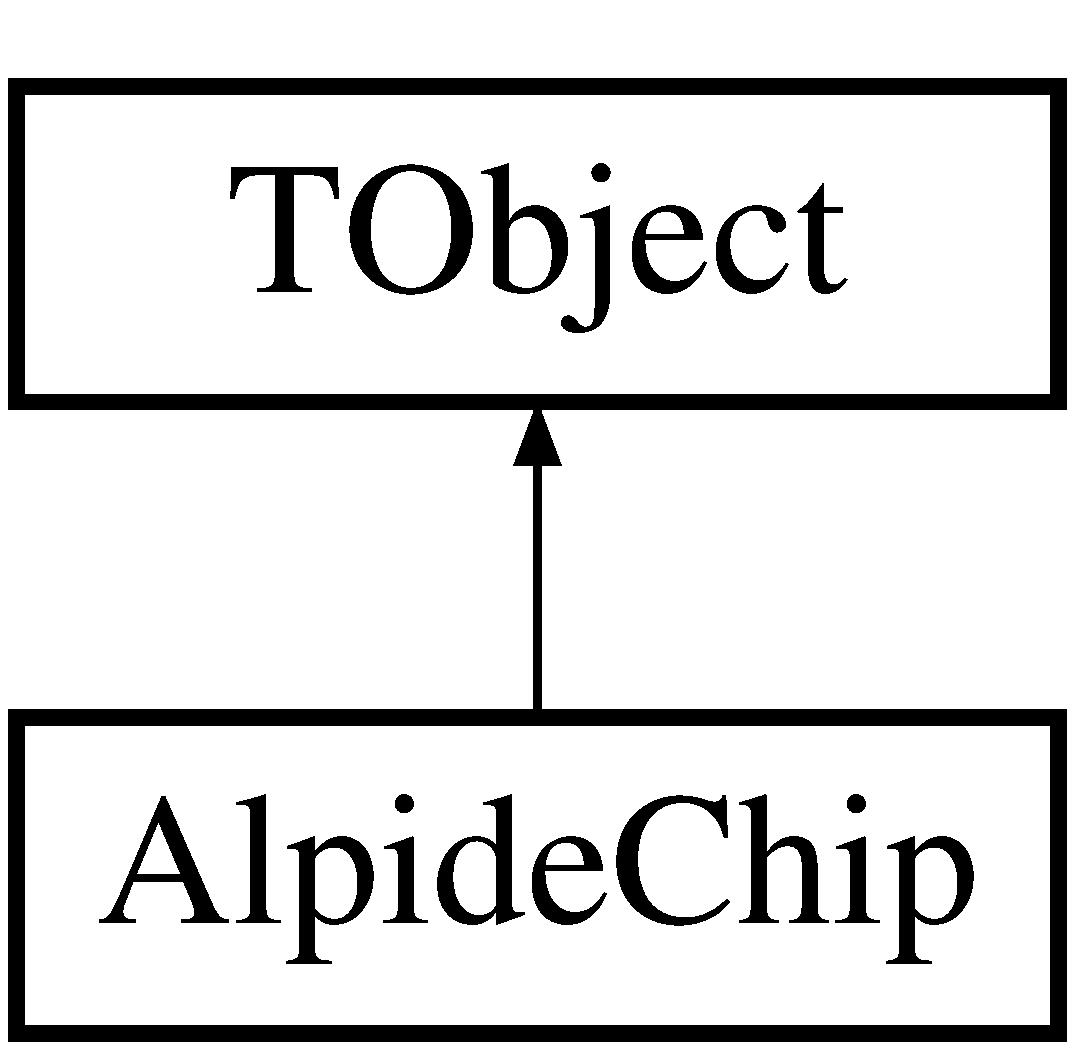
\includegraphics[height=2.000000cm]{class_alpide_chip}
\end{center}
\end{figure}
\subsection*{Public Member Functions}
\begin{DoxyCompactItemize}
\item 
\mbox{\Hypertarget{class_alpide_chip_a47ab0342d5f7c1777c30a1369cbb751f}\label{class_alpide_chip_a47ab0342d5f7c1777c30a1369cbb751f}} 
{\bfseries Alpide\+Chip} (Int\+\_\+t chip\+ID, int n\+PixelsX, int n\+PixelsY, Float\+\_\+t x\+Position, Float\+\_\+t y\+Position, Float\+\_\+t z\+Position)
\item 
\mbox{\Hypertarget{class_alpide_chip_a27394d6a941d5df23ac4173eaa6e3839}\label{class_alpide_chip_a27394d6a941d5df23ac4173eaa6e3839}} 
Int\+\_\+t {\bfseries Get\+Chip\+ID} ()
\item 
\mbox{\Hypertarget{class_alpide_chip_a4168f156f69f1100c4cfe06aef85ae95}\label{class_alpide_chip_a4168f156f69f1100c4cfe06aef85ae95}} 
T\+Clones\+Array $\ast$ {\bfseries Get\+Hit\+Pixels} () const
\item 
\mbox{\Hypertarget{class_alpide_chip_a24de2e9b8497f17a1d6a147edf0d08e3}\label{class_alpide_chip_a24de2e9b8497f17a1d6a147edf0d08e3}} 
\mbox{\hyperlink{class_alpide_pixel}{Alpide\+Pixel}} $\ast$ {\bfseries Get\+Hit\+Pixel} (Int\+\_\+t hit\+Pixel\+Index)
\item 
\mbox{\Hypertarget{class_alpide_chip_a200877fe78489ccae1d0800001288a6f}\label{class_alpide_chip_a200877fe78489ccae1d0800001288a6f}} 
\mbox{\hyperlink{class_alpide_cluster}{Alpide\+Cluster}} $\ast$ {\bfseries Get\+Cluster} (Int\+\_\+t cluster\+Index)
\item 
\mbox{\Hypertarget{class_alpide_chip_a7f33e43ee0663befd9ad50aa9ea385b4}\label{class_alpide_chip_a7f33e43ee0663befd9ad50aa9ea385b4}} 
T\+Clones\+Array $\ast$ {\bfseries Get\+Clusters} () const
\item 
\mbox{\Hypertarget{class_alpide_chip_a6e6b7a48b667c842de38795a9e1d2da2}\label{class_alpide_chip_a6e6b7a48b667c842de38795a9e1d2da2}} 
Int\+\_\+t {\bfseries Get\+Number\+Of\+Clusters} () const
\item 
\mbox{\Hypertarget{class_alpide_chip_a79d2452071a75349b4b10d76255b5216}\label{class_alpide_chip_a79d2452071a75349b4b10d76255b5216}} 
Int\+\_\+t {\bfseries Get\+Number\+Of\+PixelsX} () const
\item 
\mbox{\Hypertarget{class_alpide_chip_a781488dc5a30088419a67d6a1afec305}\label{class_alpide_chip_a781488dc5a30088419a67d6a1afec305}} 
Int\+\_\+t {\bfseries Get\+Number\+Of\+PixelsY} () const
\item 
\mbox{\Hypertarget{class_alpide_chip_a07ff24a6d35b6ad3cf110dccd5b3f063}\label{class_alpide_chip_a07ff24a6d35b6ad3cf110dccd5b3f063}} 
Int\+\_\+t {\bfseries Get\+Number\+Of\+Hit\+Pixels} () const
\item 
\mbox{\Hypertarget{class_alpide_chip_a55aa901d6df4c783b1d3186f40fbda7c}\label{class_alpide_chip_a55aa901d6df4c783b1d3186f40fbda7c}} 
Float\+\_\+t {\bfseries Get\+PositionX} () const
\item 
\mbox{\Hypertarget{class_alpide_chip_a902b95e39222ad1cef2fd5a8ff49d4ef}\label{class_alpide_chip_a902b95e39222ad1cef2fd5a8ff49d4ef}} 
Float\+\_\+t {\bfseries Get\+PositionY} () const
\item 
\mbox{\Hypertarget{class_alpide_chip_af39e802238e96b435cf11bf2ea525df8}\label{class_alpide_chip_af39e802238e96b435cf11bf2ea525df8}} 
Float\+\_\+t {\bfseries Get\+PositionZ} () const
\item 
\mbox{\Hypertarget{class_alpide_chip_a8c13f5d580acdcd12d3c7ab2bba1d23d}\label{class_alpide_chip_a8c13f5d580acdcd12d3c7ab2bba1d23d}} 
Float\+\_\+t {\bfseries Get\+SizeX} () const
\item 
\mbox{\Hypertarget{class_alpide_chip_af5b335f8c7c4368c62fcae89e0fb8ab7}\label{class_alpide_chip_af5b335f8c7c4368c62fcae89e0fb8ab7}} 
Float\+\_\+t {\bfseries Get\+SizeY} () const
\item 
\mbox{\Hypertarget{class_alpide_chip_a4859ba061f313324df3f9e0cdd726e5e}\label{class_alpide_chip_a4859ba061f313324df3f9e0cdd726e5e}} 
Float\+\_\+t {\bfseries Get\+Init\+ResoX} () const
\item 
\mbox{\Hypertarget{class_alpide_chip_a6f8680e18f2186336d2ca9a0d072022d}\label{class_alpide_chip_a6f8680e18f2186336d2ca9a0d072022d}} 
Float\+\_\+t {\bfseries Get\+Init\+ResoY} () const
\item 
\mbox{\Hypertarget{class_alpide_chip_ad2288e91351961807dd06fcd3c142294}\label{class_alpide_chip_ad2288e91351961807dd06fcd3c142294}} 
Float\+\_\+t {\bfseries Get\+Mis\+AlignX} () const
\item 
\mbox{\Hypertarget{class_alpide_chip_a387d81f517c121216861616e581e4eec}\label{class_alpide_chip_a387d81f517c121216861616e581e4eec}} 
Float\+\_\+t {\bfseries Get\+Mis\+AlignY} () const
\item 
\mbox{\Hypertarget{class_alpide_chip_aefb7feee0ce474264762a30aa2f3adc7}\label{class_alpide_chip_aefb7feee0ce474264762a30aa2f3adc7}} 
Int\+\_\+t {\bfseries Get\+Origin\+Col} () const
\item 
\mbox{\Hypertarget{class_alpide_chip_a053a1bd8a73fdf4235108bc51f7cc386}\label{class_alpide_chip_a053a1bd8a73fdf4235108bc51f7cc386}} 
Int\+\_\+t {\bfseries Get\+Origin\+Row} () const
\item 
\mbox{\Hypertarget{class_alpide_chip_af03936d0a380506bb9a893cd88ba42da}\label{class_alpide_chip_af03936d0a380506bb9a893cd88ba42da}} 
Double\+\_\+t {\bfseries Get\+Pixel\+SizeX} () const
\item 
\mbox{\Hypertarget{class_alpide_chip_a5866e6bf00d37b60acaf7de3bce2c681}\label{class_alpide_chip_a5866e6bf00d37b60acaf7de3bce2c681}} 
Double\+\_\+t {\bfseries Get\+Pixel\+SizeY} () const
\item 
\mbox{\Hypertarget{class_alpide_chip_a7870659402d0f693100083a1f50f65fb}\label{class_alpide_chip_a7870659402d0f693100083a1f50f65fb}} 
void {\bfseries Set\+Chip\+ID} (Int\+\_\+t chip\+ID)
\item 
\mbox{\Hypertarget{class_alpide_chip_ad4499363fc850f0f35ea188516fafb69}\label{class_alpide_chip_ad4499363fc850f0f35ea188516fafb69}} 
void {\bfseries Set\+Number\+Of\+PixelsX} (Int\+\_\+t n\+PixelsX)
\item 
\mbox{\Hypertarget{class_alpide_chip_a1fc034718d54e1a16bfa83a5da559961}\label{class_alpide_chip_a1fc034718d54e1a16bfa83a5da559961}} 
void {\bfseries Set\+Number\+Of\+PixelsY} (Int\+\_\+t n\+PixelsY)
\item 
\mbox{\Hypertarget{class_alpide_chip_ab19f727bac37650c8bbf4fb00a7d3691}\label{class_alpide_chip_ab19f727bac37650c8bbf4fb00a7d3691}} 
void {\bfseries Set\+Number\+Of\+Hit\+Pixels} (Int\+\_\+t n\+Hit\+Pixels)
\item 
\mbox{\Hypertarget{class_alpide_chip_ace84e19980533e95cf9c8f3bde45c671}\label{class_alpide_chip_ace84e19980533e95cf9c8f3bde45c671}} 
void {\bfseries Set\+PositionX} (Float\+\_\+t x\+Position)
\item 
\mbox{\Hypertarget{class_alpide_chip_ab75304136deab8b87f670cd00ceda3b0}\label{class_alpide_chip_ab75304136deab8b87f670cd00ceda3b0}} 
void {\bfseries Set\+PositionY} (Float\+\_\+t y\+Position)
\item 
\mbox{\Hypertarget{class_alpide_chip_a36af337accbf79dc0f0459d726a307d8}\label{class_alpide_chip_a36af337accbf79dc0f0459d726a307d8}} 
void {\bfseries Set\+PositionZ} (Float\+\_\+t z\+Position)
\item 
\mbox{\Hypertarget{class_alpide_chip_a0643c1386f818737074a65aed5466a65}\label{class_alpide_chip_a0643c1386f818737074a65aed5466a65}} 
void {\bfseries Set\+SizeX} (Float\+\_\+t x\+Size)
\item 
\mbox{\Hypertarget{class_alpide_chip_a0e3ea65ee1717efedd3c2a9caa8a704e}\label{class_alpide_chip_a0e3ea65ee1717efedd3c2a9caa8a704e}} 
void {\bfseries Set\+SizeY} (Float\+\_\+t y\+Size)
\item 
\mbox{\Hypertarget{class_alpide_chip_a6232718f762cabbc6fe5be2a40aae831}\label{class_alpide_chip_a6232718f762cabbc6fe5be2a40aae831}} 
void {\bfseries Set\+Init\+ResoX} (Float\+\_\+t x\+Reso)
\item 
\mbox{\Hypertarget{class_alpide_chip_a58c4c96f9b7f2d7321ec247f625851cc}\label{class_alpide_chip_a58c4c96f9b7f2d7321ec247f625851cc}} 
void {\bfseries Set\+Init\+ResoY} (Float\+\_\+t y\+Reso)
\item 
\mbox{\Hypertarget{class_alpide_chip_ada005001e84d8670cb0d50fc44cf0dfd}\label{class_alpide_chip_ada005001e84d8670cb0d50fc44cf0dfd}} 
void {\bfseries Set\+Mis\+AlignX} (Float\+\_\+t x\+Mis\+Align)
\item 
\mbox{\Hypertarget{class_alpide_chip_aed00efb46ae3f064bc5bd84a2cf4472b}\label{class_alpide_chip_aed00efb46ae3f064bc5bd84a2cf4472b}} 
void {\bfseries Set\+Mis\+AlignY} (Float\+\_\+t y\+Mis\+Align)
\item 
\mbox{\Hypertarget{class_alpide_chip_a265b22345579c7cec8a3f31bfa79068a}\label{class_alpide_chip_a265b22345579c7cec8a3f31bfa79068a}} 
void {\bfseries Set\+Origin\+Col} (Int\+\_\+t col)
\item 
\mbox{\Hypertarget{class_alpide_chip_add081ad7aa40e72831514519a16ea9c1}\label{class_alpide_chip_add081ad7aa40e72831514519a16ea9c1}} 
void {\bfseries Set\+Origin\+Row} (Int\+\_\+t row)
\item 
\mbox{\Hypertarget{class_alpide_chip_a904459d8273bc0177c6b25ce38094a7d}\label{class_alpide_chip_a904459d8273bc0177c6b25ce38094a7d}} 
void {\bfseries Set\+Pixel\+SizeX} (Int\+\_\+t x\+Size)
\item 
\mbox{\Hypertarget{class_alpide_chip_a3d41d2683ed3ef2a5af33c985c364d98}\label{class_alpide_chip_a3d41d2683ed3ef2a5af33c985c364d98}} 
void {\bfseries Set\+Pixel\+SizeY} (Int\+\_\+t y\+Size)
\item 
\mbox{\Hypertarget{class_alpide_chip_a89a004c008c7c7970c261df38036dfdd}\label{class_alpide_chip_a89a004c008c7c7970c261df38036dfdd}} 
void {\bfseries Add\+Cluster} (\mbox{\hyperlink{class_alpide_cluster}{Alpide\+Cluster}} $\ast$cluster)
\item 
\mbox{\Hypertarget{class_alpide_chip_a2d0271bb015324f6181e67819e5da692}\label{class_alpide_chip_a2d0271bb015324f6181e67819e5da692}} 
void {\bfseries Add\+Hit\+Pixel} (\mbox{\hyperlink{class_alpide_pixel}{Alpide\+Pixel}} $\ast$pixel)
\item 
\mbox{\Hypertarget{class_alpide_chip_ac6074ffa77d278d1f42e6d47e1c740e0}\label{class_alpide_chip_ac6074ffa77d278d1f42e6d47e1c740e0}} 
Bool\+\_\+t {\bfseries Is\+A\+Point\+In\+A\+Cluster} (Float\+\_\+t x\+Coordinate, Float\+\_\+t y\+Coordinate, Int\+\_\+t \&cluster\+Index)
\item 
\mbox{\Hypertarget{class_alpide_chip_a993814fa745c75cc72fc28e758a08d5e}\label{class_alpide_chip_a993814fa745c75cc72fc28e758a08d5e}} 
void {\bfseries Clusters\+Rec\+In\+Chip} ()
\item 
\mbox{\Hypertarget{class_alpide_chip_aaeb6c6d98741407f7a6d0834476cd359}\label{class_alpide_chip_aaeb6c6d98741407f7a6d0834476cd359}} 
void {\bfseries Reset\+Chip} ()
\item 
\mbox{\Hypertarget{class_alpide_chip_aba0d7fcac933f1a7012649338432b623}\label{class_alpide_chip_aba0d7fcac933f1a7012649338432b623}} 
{\bfseries Class\+Def} (\mbox{\hyperlink{class_alpide_chip}{Alpide\+Chip}}, 1)
\end{DoxyCompactItemize}
\subsection*{Private Attributes}
\begin{DoxyCompactItemize}
\item 
\mbox{\Hypertarget{class_alpide_chip_a4ce9880ecd33c67266b22cd130a3e557}\label{class_alpide_chip_a4ce9880ecd33c67266b22cd130a3e557}} 
Int\+\_\+t {\bfseries f\+Chip\+ID}
\item 
\mbox{\Hypertarget{class_alpide_chip_a0ba09bd7a3c6951c63c58054d7de4afe}\label{class_alpide_chip_a0ba09bd7a3c6951c63c58054d7de4afe}} 
Int\+\_\+t {\bfseries f\+Number\+Of\+PixelsX}
\item 
\mbox{\Hypertarget{class_alpide_chip_adcdcda4d5b53a02ffdf634c77b08b59c}\label{class_alpide_chip_adcdcda4d5b53a02ffdf634c77b08b59c}} 
Int\+\_\+t {\bfseries f\+Number\+Of\+PixelsY}
\item 
\mbox{\Hypertarget{class_alpide_chip_a44de2af2161a7472931b0b9e11915816}\label{class_alpide_chip_a44de2af2161a7472931b0b9e11915816}} 
Float\+\_\+t {\bfseries f\+Chip\+PositionX}
\item 
\mbox{\Hypertarget{class_alpide_chip_a2d0cff27c76736c76166c45eebc19b3e}\label{class_alpide_chip_a2d0cff27c76736c76166c45eebc19b3e}} 
Float\+\_\+t {\bfseries f\+Chip\+PositionY}
\item 
\mbox{\Hypertarget{class_alpide_chip_a1715a6f5fa914055cfb9dd2c4aa126f9}\label{class_alpide_chip_a1715a6f5fa914055cfb9dd2c4aa126f9}} 
Float\+\_\+t {\bfseries f\+Chip\+PositionZ}
\item 
\mbox{\Hypertarget{class_alpide_chip_aff13a859785899c92b89a20f61b31c06}\label{class_alpide_chip_aff13a859785899c92b89a20f61b31c06}} 
Float\+\_\+t {\bfseries f\+Chip\+SizeX}
\item 
\mbox{\Hypertarget{class_alpide_chip_abef2b4a5c566837b3d62c740f9610ba4}\label{class_alpide_chip_abef2b4a5c566837b3d62c740f9610ba4}} 
Float\+\_\+t {\bfseries f\+Chip\+SizeY}
\item 
\mbox{\Hypertarget{class_alpide_chip_a18aa2ae88cec1aef589b0c1380ffcea7}\label{class_alpide_chip_a18aa2ae88cec1aef589b0c1380ffcea7}} 
Float\+\_\+t {\bfseries f\+Chip\+Init\+ResoX}
\item 
\mbox{\Hypertarget{class_alpide_chip_a52e79e3f03e63ae7b23c294e08ff1ece}\label{class_alpide_chip_a52e79e3f03e63ae7b23c294e08ff1ece}} 
Float\+\_\+t {\bfseries f\+Chip\+Init\+ResoY}
\item 
\mbox{\Hypertarget{class_alpide_chip_a1c0ac447704be162766e940f69b04834}\label{class_alpide_chip_a1c0ac447704be162766e940f69b04834}} 
Float\+\_\+t {\bfseries f\+Mis\+AlignX}
\item 
\mbox{\Hypertarget{class_alpide_chip_ac0d77515f4546759efeb8a9a139664b4}\label{class_alpide_chip_ac0d77515f4546759efeb8a9a139664b4}} 
Float\+\_\+t {\bfseries f\+Mis\+AlignY}
\item 
\mbox{\Hypertarget{class_alpide_chip_ab92d8630c0056a1ab5b9cce78ec872e2}\label{class_alpide_chip_ab92d8630c0056a1ab5b9cce78ec872e2}} 
Int\+\_\+t {\bfseries f\+Origin\+Col}
\item 
\mbox{\Hypertarget{class_alpide_chip_a258d547d2e5d3323be237577d5d9b714}\label{class_alpide_chip_a258d547d2e5d3323be237577d5d9b714}} 
Int\+\_\+t {\bfseries f\+Origin\+Row}
\item 
\mbox{\Hypertarget{class_alpide_chip_a80cb51a5a2779d04fb9edcada89f8351}\label{class_alpide_chip_a80cb51a5a2779d04fb9edcada89f8351}} 
Double\+\_\+t {\bfseries f\+Pixel\+SizeX}
\item 
\mbox{\Hypertarget{class_alpide_chip_a60a7359c897973e1bb7b6a51311789fe}\label{class_alpide_chip_a60a7359c897973e1bb7b6a51311789fe}} 
Double\+\_\+t {\bfseries f\+Pixel\+SizeY}
\item 
\mbox{\Hypertarget{class_alpide_chip_ae22a1320224247feac437e9351b0f6d3}\label{class_alpide_chip_ae22a1320224247feac437e9351b0f6d3}} 
Int\+\_\+t {\bfseries f\+Number\+Of\+Hit\+Pixels}
\item 
\mbox{\Hypertarget{class_alpide_chip_a4c5e70de283159303935b92fec1b6635}\label{class_alpide_chip_a4c5e70de283159303935b92fec1b6635}} 
T\+Clones\+Array $\ast$ {\bfseries f\+Array\+Hit\+Pixels}
\item 
\mbox{\Hypertarget{class_alpide_chip_a0fc4b7bcc6be9bad820417d35852c92c}\label{class_alpide_chip_a0fc4b7bcc6be9bad820417d35852c92c}} 
Int\+\_\+t {\bfseries f\+Number\+Of\+Clusters}
\item 
\mbox{\Hypertarget{class_alpide_chip_abee2713286d7237e8033df54181f3bfb}\label{class_alpide_chip_abee2713286d7237e8033df54181f3bfb}} 
T\+Clones\+Array $\ast$ {\bfseries f\+Array\+Clusters}
\end{DoxyCompactItemize}


The documentation for this class was generated from the following files\+:\begin{DoxyCompactItemize}
\item 
/\+Users/tarhini/\+Desktop/\+M\+F\+T/test\+Beam\+Analysis/my-\/\+M\+F\+T-\/\+Analysis/src/Alpide\+Chip.\+hpp\item 
/\+Users/tarhini/\+Desktop/\+M\+F\+T/test\+Beam\+Analysis/my-\/\+M\+F\+T-\/\+Analysis/src/Alpide\+Chip.\+cpp\end{DoxyCompactItemize}

\hypertarget{class_alpide_cluster}{}\section{Alpide\+Cluster Class Reference}
\label{class_alpide_cluster}\index{Alpide\+Cluster@{Alpide\+Cluster}}
Inheritance diagram for Alpide\+Cluster\+:\begin{figure}[H]
\begin{center}
\leavevmode
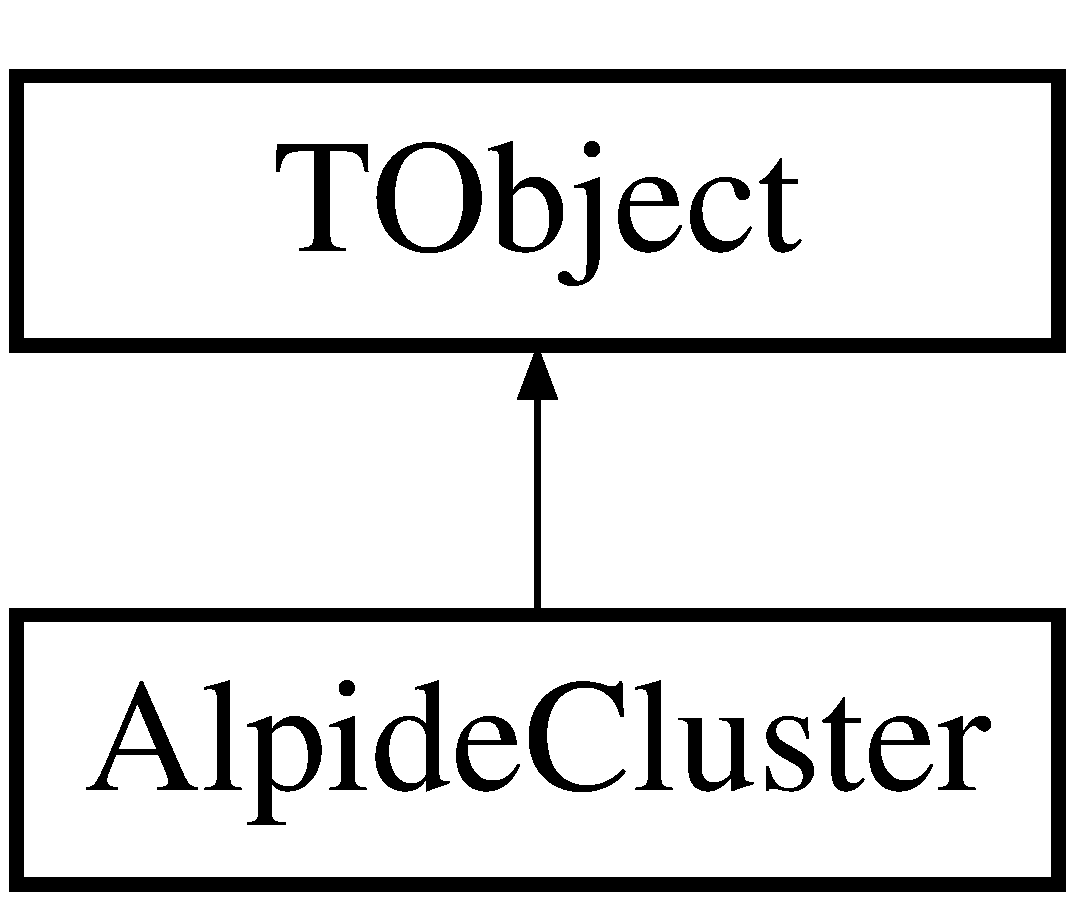
\includegraphics[height=2.000000cm]{class_alpide_cluster}
\end{center}
\end{figure}
\subsection*{Public Member Functions}
\begin{DoxyCompactItemize}
\item 
\mbox{\Hypertarget{class_alpide_cluster_af821b31fed68e996a6bb53c373687efc}\label{class_alpide_cluster_af821b31fed68e996a6bb53c373687efc}} 
{\bfseries Alpide\+Cluster} (Int\+\_\+t n\+Pixels)
\item 
\mbox{\Hypertarget{class_alpide_cluster_a008fae4dd8d87b1f5b21c308628cfaff}\label{class_alpide_cluster_a008fae4dd8d87b1f5b21c308628cfaff}} 
Int\+\_\+t {\bfseries Get\+Number\+Of\+Pixels} () const
\item 
\mbox{\Hypertarget{class_alpide_cluster_adb8cc438b171a4caba741eaed62a6839}\label{class_alpide_cluster_adb8cc438b171a4caba741eaed62a6839}} 
T\+Clones\+Array $\ast$ {\bfseries Get\+Pixel\+Array} () const
\item 
\mbox{\Hypertarget{class_alpide_cluster_a007d219e1928cc3f5625565cab061d37}\label{class_alpide_cluster_a007d219e1928cc3f5625565cab061d37}} 
\mbox{\hyperlink{class_alpide_pixel}{Alpide\+Pixel}} $\ast$ {\bfseries Get\+Pixel} (Int\+\_\+t pixel\+Index)
\item 
Int\+\_\+t \mbox{\hyperlink{class_alpide_cluster_ae55b212b27e3675ae39fefe0609e64bc}{Get\+Center\+Of\+Mass\+Col}} ()
\item 
Int\+\_\+t \mbox{\hyperlink{class_alpide_cluster_aa6a01c099653dc06d5b9b4dbbbc0bd40}{Get\+Center\+Of\+Mass\+Row}} ()
\item 
Int\+\_\+t \mbox{\hyperlink{class_alpide_cluster_afcca84fccea029577b9c6000b9150ca7}{Get\+Col\+Spread}} ()
\item 
Int\+\_\+t \mbox{\hyperlink{class_alpide_cluster_a3a013131ed160c17cace1ba9390678f7}{Get\+Row\+Spread}} ()
\item 
Int\+\_\+t \mbox{\hyperlink{class_alpide_cluster_ad956ba719becb064aa333b53b5e8044e}{Get\+Total\+Spread}} ()
\item 
\mbox{\Hypertarget{class_alpide_cluster_a17c57fda1cdece3403a5cca96b9b8554}\label{class_alpide_cluster_a17c57fda1cdece3403a5cca96b9b8554}} 
Double\+\_\+t {\bfseries Get\+Center\+Of\+MassX} () const
\item 
\mbox{\Hypertarget{class_alpide_cluster_a13544622bdc93308485b97b8aaf27c75}\label{class_alpide_cluster_a13544622bdc93308485b97b8aaf27c75}} 
Double\+\_\+t {\bfseries Get\+Center\+Of\+MassY} () const
\item 
\mbox{\Hypertarget{class_alpide_cluster_ac32c99edeb62efba4431fe74ea07df6f}\label{class_alpide_cluster_ac32c99edeb62efba4431fe74ea07df6f}} 
Double\+\_\+t {\bfseries Get\+SpreadX} () const
\item 
\mbox{\Hypertarget{class_alpide_cluster_a6d567c91d25d698075c267d96f5c83e6}\label{class_alpide_cluster_a6d567c91d25d698075c267d96f5c83e6}} 
Double\+\_\+t {\bfseries Get\+SpreadY} () const
\item 
\mbox{\Hypertarget{class_alpide_cluster_a2a5250947ca4f2505c156fa8755a72c1}\label{class_alpide_cluster_a2a5250947ca4f2505c156fa8755a72c1}} 
void {\bfseries Set\+Center\+Of\+MassX} (Double\+\_\+t x)
\item 
\mbox{\Hypertarget{class_alpide_cluster_a24326db8f7e7a36f46523f4031c3c995}\label{class_alpide_cluster_a24326db8f7e7a36f46523f4031c3c995}} 
void {\bfseries Set\+Center\+Of\+MassY} (Double\+\_\+t y)
\item 
\mbox{\Hypertarget{class_alpide_cluster_acc51c586b7d86dd19e1fe7f0842901e7}\label{class_alpide_cluster_acc51c586b7d86dd19e1fe7f0842901e7}} 
void {\bfseries Set\+SpreadX} (Double\+\_\+t x)
\item 
\mbox{\Hypertarget{class_alpide_cluster_ac41e6bb51f42f81da59a3e0a4d83a91a}\label{class_alpide_cluster_ac41e6bb51f42f81da59a3e0a4d83a91a}} 
void {\bfseries Set\+SpreadY} (Double\+\_\+t y)
\item 
\mbox{\Hypertarget{class_alpide_cluster_a8fb86aad62f5e9bcdfdf70ccf0512ed0}\label{class_alpide_cluster_a8fb86aad62f5e9bcdfdf70ccf0512ed0}} 
void {\bfseries Add\+Pixel} (\mbox{\hyperlink{class_alpide_pixel}{Alpide\+Pixel}} $\ast$pixel)
\item 
\mbox{\Hypertarget{class_alpide_cluster_adde177ceced7edb8b8ecde3c05043186}\label{class_alpide_cluster_adde177ceced7edb8b8ecde3c05043186}} 
Bool\+\_\+t {\bfseries Is\+Pixel\+Touch\+The\+Cluster} (\mbox{\hyperlink{class_alpide_pixel}{Alpide\+Pixel}} $\ast$pixel)
\item 
\mbox{\Hypertarget{class_alpide_cluster_a37055d9d43c3961a6439d56bbfe7d4c3}\label{class_alpide_cluster_a37055d9d43c3961a6439d56bbfe7d4c3}} 
void {\bfseries Reset\+Cluster} ()
\item 
\mbox{\Hypertarget{class_alpide_cluster_ad7daeae5887cd6598afa9da94e06c1b2}\label{class_alpide_cluster_ad7daeae5887cd6598afa9da94e06c1b2}} 
{\bfseries Class\+Def} (\mbox{\hyperlink{class_alpide_cluster}{Alpide\+Cluster}}, 2)
\end{DoxyCompactItemize}
\subsection*{Private Attributes}
\begin{DoxyCompactItemize}
\item 
Int\+\_\+t \mbox{\hyperlink{class_alpide_cluster_a201c3e825ff2d703e7d18d05c801495d}{f\+Number\+Of\+Pixels}}
\item 
\mbox{\Hypertarget{class_alpide_cluster_a5a85490b4de8928b3fb1f46bd0303215}\label{class_alpide_cluster_a5a85490b4de8928b3fb1f46bd0303215}} 
T\+Clones\+Array $\ast$ {\bfseries f\+Array\+Pixels}
\item 
\mbox{\Hypertarget{class_alpide_cluster_a10d6502e45adde8d36589033dcbf5846}\label{class_alpide_cluster_a10d6502e45adde8d36589033dcbf5846}} 
Double\+\_\+t {\bfseries f\+Center\+Of\+MassX}
\item 
\mbox{\Hypertarget{class_alpide_cluster_a1925a67ccc2a7543facb3e3131ff9f16}\label{class_alpide_cluster_a1925a67ccc2a7543facb3e3131ff9f16}} 
Double\+\_\+t {\bfseries f\+Center\+Of\+MassY}
\item 
\mbox{\Hypertarget{class_alpide_cluster_adabdacb6a49b339e829f87c41ddb81cf}\label{class_alpide_cluster_adabdacb6a49b339e829f87c41ddb81cf}} 
Double\+\_\+t {\bfseries f\+SpreadX}
\item 
\mbox{\Hypertarget{class_alpide_cluster_af0f6a4e861d7ba9ec2e7860c33dcf372}\label{class_alpide_cluster_af0f6a4e861d7ba9ec2e7860c33dcf372}} 
Double\+\_\+t {\bfseries f\+SpreadY}
\end{DoxyCompactItemize}


\subsection{Member Function Documentation}
\mbox{\Hypertarget{class_alpide_cluster_ae55b212b27e3675ae39fefe0609e64bc}\label{class_alpide_cluster_ae55b212b27e3675ae39fefe0609e64bc}} 
\index{Alpide\+Cluster@{Alpide\+Cluster}!Get\+Center\+Of\+Mass\+Col@{Get\+Center\+Of\+Mass\+Col}}
\index{Get\+Center\+Of\+Mass\+Col@{Get\+Center\+Of\+Mass\+Col}!Alpide\+Cluster@{Alpide\+Cluster}}
\subsubsection{\texorpdfstring{Get\+Center\+Of\+Mass\+Col()}{GetCenterOfMassCol()}}
{\footnotesize\ttfamily Int\+\_\+t Alpide\+Cluster\+::\+Get\+Center\+Of\+Mass\+Col (\begin{DoxyParamCaption}{ }\end{DoxyParamCaption})}

X position of c.\+m. of cluster signal. For the moment, the weight of each hit is 1 . (right ?) \mbox{\Hypertarget{class_alpide_cluster_aa6a01c099653dc06d5b9b4dbbbc0bd40}\label{class_alpide_cluster_aa6a01c099653dc06d5b9b4dbbbc0bd40}} 
\index{Alpide\+Cluster@{Alpide\+Cluster}!Get\+Center\+Of\+Mass\+Row@{Get\+Center\+Of\+Mass\+Row}}
\index{Get\+Center\+Of\+Mass\+Row@{Get\+Center\+Of\+Mass\+Row}!Alpide\+Cluster@{Alpide\+Cluster}}
\subsubsection{\texorpdfstring{Get\+Center\+Of\+Mass\+Row()}{GetCenterOfMassRow()}}
{\footnotesize\ttfamily Int\+\_\+t Alpide\+Cluster\+::\+Get\+Center\+Of\+Mass\+Row (\begin{DoxyParamCaption}{ }\end{DoxyParamCaption})}

Y position of c.\+m. of cluster signal \mbox{\Hypertarget{class_alpide_cluster_afcca84fccea029577b9c6000b9150ca7}\label{class_alpide_cluster_afcca84fccea029577b9c6000b9150ca7}} 
\index{Alpide\+Cluster@{Alpide\+Cluster}!Get\+Col\+Spread@{Get\+Col\+Spread}}
\index{Get\+Col\+Spread@{Get\+Col\+Spread}!Alpide\+Cluster@{Alpide\+Cluster}}
\subsubsection{\texorpdfstring{Get\+Col\+Spread()}{GetColSpread()}}
{\footnotesize\ttfamily Int\+\_\+t Alpide\+Cluster\+::\+Get\+Col\+Spread (\begin{DoxyParamCaption}{ }\end{DoxyParamCaption})}

the max x-\/distance between the pixels \mbox{\Hypertarget{class_alpide_cluster_a3a013131ed160c17cace1ba9390678f7}\label{class_alpide_cluster_a3a013131ed160c17cace1ba9390678f7}} 
\index{Alpide\+Cluster@{Alpide\+Cluster}!Get\+Row\+Spread@{Get\+Row\+Spread}}
\index{Get\+Row\+Spread@{Get\+Row\+Spread}!Alpide\+Cluster@{Alpide\+Cluster}}
\subsubsection{\texorpdfstring{Get\+Row\+Spread()}{GetRowSpread()}}
{\footnotesize\ttfamily Int\+\_\+t Alpide\+Cluster\+::\+Get\+Row\+Spread (\begin{DoxyParamCaption}{ }\end{DoxyParamCaption})}

the max y-\/distance between the pixels \mbox{\Hypertarget{class_alpide_cluster_ad956ba719becb064aa333b53b5e8044e}\label{class_alpide_cluster_ad956ba719becb064aa333b53b5e8044e}} 
\index{Alpide\+Cluster@{Alpide\+Cluster}!Get\+Total\+Spread@{Get\+Total\+Spread}}
\index{Get\+Total\+Spread@{Get\+Total\+Spread}!Alpide\+Cluster@{Alpide\+Cluster}}
\subsubsection{\texorpdfstring{Get\+Total\+Spread()}{GetTotalSpread()}}
{\footnotesize\ttfamily Int\+\_\+t Alpide\+Cluster\+::\+Get\+Total\+Spread (\begin{DoxyParamCaption}{ }\end{DoxyParamCaption})}

the max xy-\/distance between the pixels 

\subsection{Member Data Documentation}
\mbox{\Hypertarget{class_alpide_cluster_a201c3e825ff2d703e7d18d05c801495d}\label{class_alpide_cluster_a201c3e825ff2d703e7d18d05c801495d}} 
\index{Alpide\+Cluster@{Alpide\+Cluster}!f\+Number\+Of\+Pixels@{f\+Number\+Of\+Pixels}}
\index{f\+Number\+Of\+Pixels@{f\+Number\+Of\+Pixels}!Alpide\+Cluster@{Alpide\+Cluster}}
\subsubsection{\texorpdfstring{f\+Number\+Of\+Pixels}{fNumberOfPixels}}
{\footnotesize\ttfamily Int\+\_\+t Alpide\+Cluster\+::f\+Number\+Of\+Pixels\hspace{0.3cm}{\ttfamily [private]}}

number of hit pixels in the cluster. T\+O\+DO\+: Is there a maximum number fot the pixels in one cluster ? 

The documentation for this class was generated from the following files\+:\begin{DoxyCompactItemize}
\item 
/\+Users/tarhini/\+Desktop/\+M\+F\+T/test\+Beam\+Analysis/my-\/\+M\+F\+T-\/\+Analysis/src/Alpide\+Cluster.\+hpp\item 
/\+Users/tarhini/\+Desktop/\+M\+F\+T/test\+Beam\+Analysis/my-\/\+M\+F\+T-\/\+Analysis/src/Alpide\+Cluster.\+cpp\end{DoxyCompactItemize}

\hypertarget{class_alpide_ladder}{}\section{Alpide\+Ladder Class Reference}
\label{class_alpide_ladder}\index{Alpide\+Ladder@{Alpide\+Ladder}}


{\ttfamily \#include $<$Alpide\+Ladder.\+hpp$>$}

Inheritance diagram for Alpide\+Ladder\+:\begin{figure}[H]
\begin{center}
\leavevmode
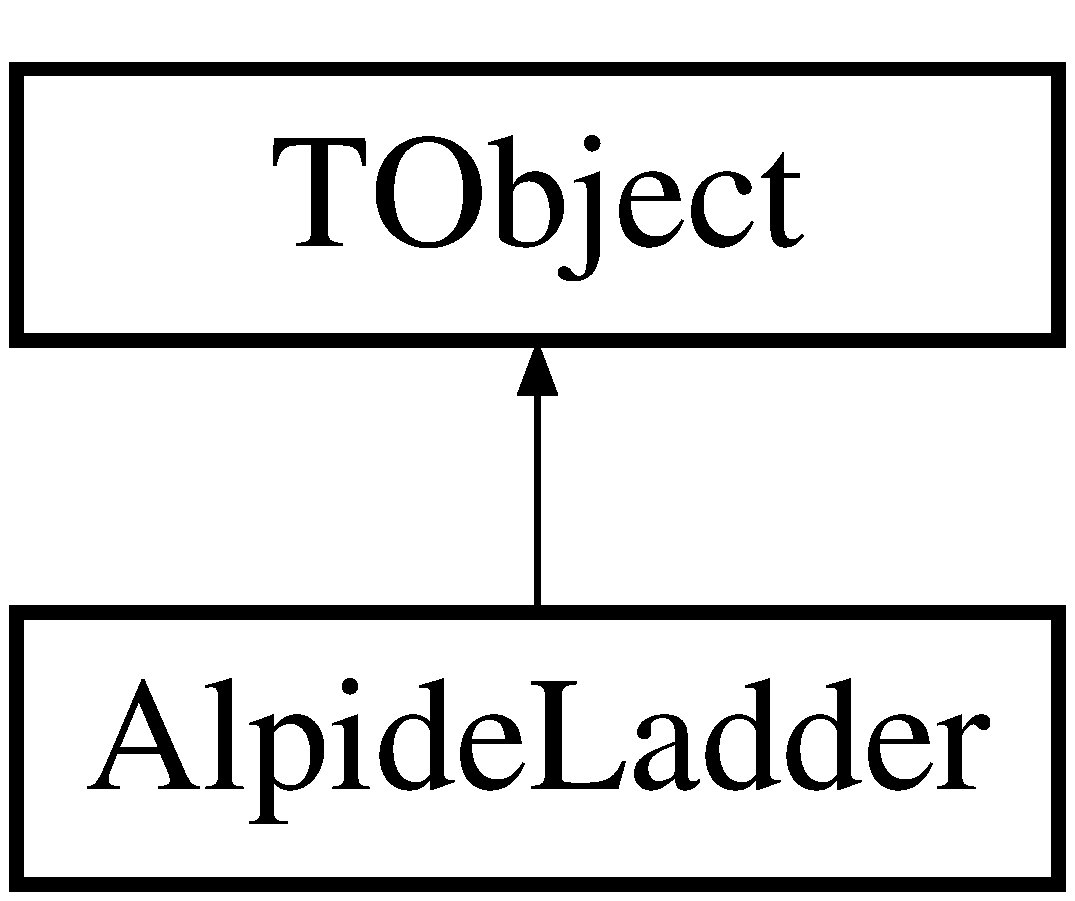
\includegraphics[height=2.000000cm]{class_alpide_ladder}
\end{center}
\end{figure}
\subsection*{Public Member Functions}
\begin{DoxyCompactItemize}
\item 
\mbox{\Hypertarget{class_alpide_ladder_a1eb68d4bca9be56454bb038050dcb636}\label{class_alpide_ladder_a1eb68d4bca9be56454bb038050dcb636}} 
{\bfseries Alpide\+Ladder} (Int\+\_\+t ladder\+ID)
\item 
\mbox{\Hypertarget{class_alpide_ladder_a094c6b21c41939556b6e2bc0e558a954}\label{class_alpide_ladder_a094c6b21c41939556b6e2bc0e558a954}} 
Int\+\_\+t {\bfseries Get\+Ladder\+ID} () const
\item 
\mbox{\Hypertarget{class_alpide_ladder_a6c897e52319dbf198e03399da9c2b006}\label{class_alpide_ladder_a6c897e52319dbf198e03399da9c2b006}} 
Int\+\_\+t {\bfseries Get\+Number\+Of\+Chips} () const
\item 
\mbox{\Hypertarget{class_alpide_ladder_a8c2000138b09528cf1b1a6237cd655d4}\label{class_alpide_ladder_a8c2000138b09528cf1b1a6237cd655d4}} 
\mbox{\hyperlink{class_alpide_chip}{Alpide\+Chip}} $\ast$ {\bfseries Get\+Chip} (Int\+\_\+t index)
\item 
\mbox{\Hypertarget{class_alpide_ladder_a14c0d9e30712e27aac188a07698ab98f}\label{class_alpide_ladder_a14c0d9e30712e27aac188a07698ab98f}} 
\mbox{\hyperlink{class_alpide_chip}{Alpide\+Chip}} $\ast$ {\bfseries Get\+Chip\+By\+ID} (Int\+\_\+t chip\+ID)
\item 
\mbox{\Hypertarget{class_alpide_ladder_a304b609bc2214bcaaa20ecc02059c087}\label{class_alpide_ladder_a304b609bc2214bcaaa20ecc02059c087}} 
T\+Clones\+Array $\ast$ {\bfseries Get\+Array\+Chips} () const
\item 
\mbox{\Hypertarget{class_alpide_ladder_a98ddc66d0678fd44709888bde9a48015}\label{class_alpide_ladder_a98ddc66d0678fd44709888bde9a48015}} 
void {\bfseries Set\+Ladder\+ID} (Int\+\_\+t ladder\+ID)
\item 
\mbox{\Hypertarget{class_alpide_ladder_a5d93d03f5253d92396e21e4f0cc6b309}\label{class_alpide_ladder_a5d93d03f5253d92396e21e4f0cc6b309}} 
void {\bfseries Add\+Chip} (\mbox{\hyperlink{class_alpide_chip}{Alpide\+Chip}} $\ast$chip)
\item 
\mbox{\Hypertarget{class_alpide_ladder_ad4538b416fc063cf2a48a5ba5df65122}\label{class_alpide_ladder_ad4538b416fc063cf2a48a5ba5df65122}} 
void {\bfseries Reset\+Ladder} ()
\item 
\mbox{\Hypertarget{class_alpide_ladder_af6d0c45740ade18d0a8bde8a90898d5b}\label{class_alpide_ladder_af6d0c45740ade18d0a8bde8a90898d5b}} 
{\bfseries Class\+Def} (\mbox{\hyperlink{class_alpide_ladder}{Alpide\+Ladder}}, 1)
\end{DoxyCompactItemize}
\subsection*{Private Attributes}
\begin{DoxyCompactItemize}
\item 
Int\+\_\+t \mbox{\hyperlink{class_alpide_ladder_a5e51ffcfae1349f109896750a8d983d4}{f\+Ladder\+ID}}
\item 
Int\+\_\+t \mbox{\hyperlink{class_alpide_ladder_a90b3940b3c8b563115cc16efa27f4478}{f\+Number\+Of\+Chips}}
\item 
T\+Clones\+Array $\ast$ \mbox{\hyperlink{class_alpide_ladder_a9539572046b2da5582019ae4f0148428}{f\+Array\+Chips}}
\end{DoxyCompactItemize}


\subsection{Detailed Description}
A class for a M\+FT ladder. The ladder contains many Alpide\+Chips (2,3,or 4). In addition to the array of chips and their number, the ladder class has an a variable that indicates whether the ladder is on the face or the back side of the disk so that the numbering of the columns can be set. T\+O\+DO\+: This class was developped before knowing that the telescope used in the test beam is also based on alpide chips, one cab think of making a detector class that can be either ladder or a telescope. 

\subsection{Member Data Documentation}
\mbox{\Hypertarget{class_alpide_ladder_a9539572046b2da5582019ae4f0148428}\label{class_alpide_ladder_a9539572046b2da5582019ae4f0148428}} 
\index{Alpide\+Ladder@{Alpide\+Ladder}!f\+Array\+Chips@{f\+Array\+Chips}}
\index{f\+Array\+Chips@{f\+Array\+Chips}!Alpide\+Ladder@{Alpide\+Ladder}}
\subsubsection{\texorpdfstring{f\+Array\+Chips}{fArrayChips}}
{\footnotesize\ttfamily T\+Clones\+Array$\ast$ Alpide\+Ladder\+::f\+Array\+Chips\hspace{0.3cm}{\ttfamily [private]}}

A vector of chips can be used but tobjarray may be more flexible in the further analysis. \mbox{\Hypertarget{class_alpide_ladder_a5e51ffcfae1349f109896750a8d983d4}\label{class_alpide_ladder_a5e51ffcfae1349f109896750a8d983d4}} 
\index{Alpide\+Ladder@{Alpide\+Ladder}!f\+Ladder\+ID@{f\+Ladder\+ID}}
\index{f\+Ladder\+ID@{f\+Ladder\+ID}!Alpide\+Ladder@{Alpide\+Ladder}}
\subsubsection{\texorpdfstring{f\+Ladder\+ID}{fLadderID}}
{\footnotesize\ttfamily Int\+\_\+t Alpide\+Ladder\+::f\+Ladder\+ID\hspace{0.3cm}{\ttfamily [private]}}

This id must match the id system in the raw file \mbox{\Hypertarget{class_alpide_ladder_a90b3940b3c8b563115cc16efa27f4478}\label{class_alpide_ladder_a90b3940b3c8b563115cc16efa27f4478}} 
\index{Alpide\+Ladder@{Alpide\+Ladder}!f\+Number\+Of\+Chips@{f\+Number\+Of\+Chips}}
\index{f\+Number\+Of\+Chips@{f\+Number\+Of\+Chips}!Alpide\+Ladder@{Alpide\+Ladder}}
\subsubsection{\texorpdfstring{f\+Number\+Of\+Chips}{fNumberOfChips}}
{\footnotesize\ttfamily Int\+\_\+t Alpide\+Ladder\+::f\+Number\+Of\+Chips\hspace{0.3cm}{\ttfamily [private]}}

number of chips in the ladder. 

The documentation for this class was generated from the following files\+:\begin{DoxyCompactItemize}
\item 
/\+Users/tarhini/\+Desktop/\+M\+F\+T/test\+Beam\+Analysis/my-\/\+M\+F\+T-\/\+Analysis/src/Alpide\+Ladder.\+hpp\item 
/\+Users/tarhini/\+Desktop/\+M\+F\+T/test\+Beam\+Analysis/my-\/\+M\+F\+T-\/\+Analysis/src/Alpide\+Ladder.\+cpp\end{DoxyCompactItemize}

\hypertarget{class_alpide_pixel}{}\section{Alpide\+Pixel Class Reference}
\label{class_alpide_pixel}\index{Alpide\+Pixel@{Alpide\+Pixel}}


{\ttfamily \#include $<$Alpide\+Pixel.\+hpp$>$}

Inheritance diagram for Alpide\+Pixel\+:\begin{figure}[H]
\begin{center}
\leavevmode
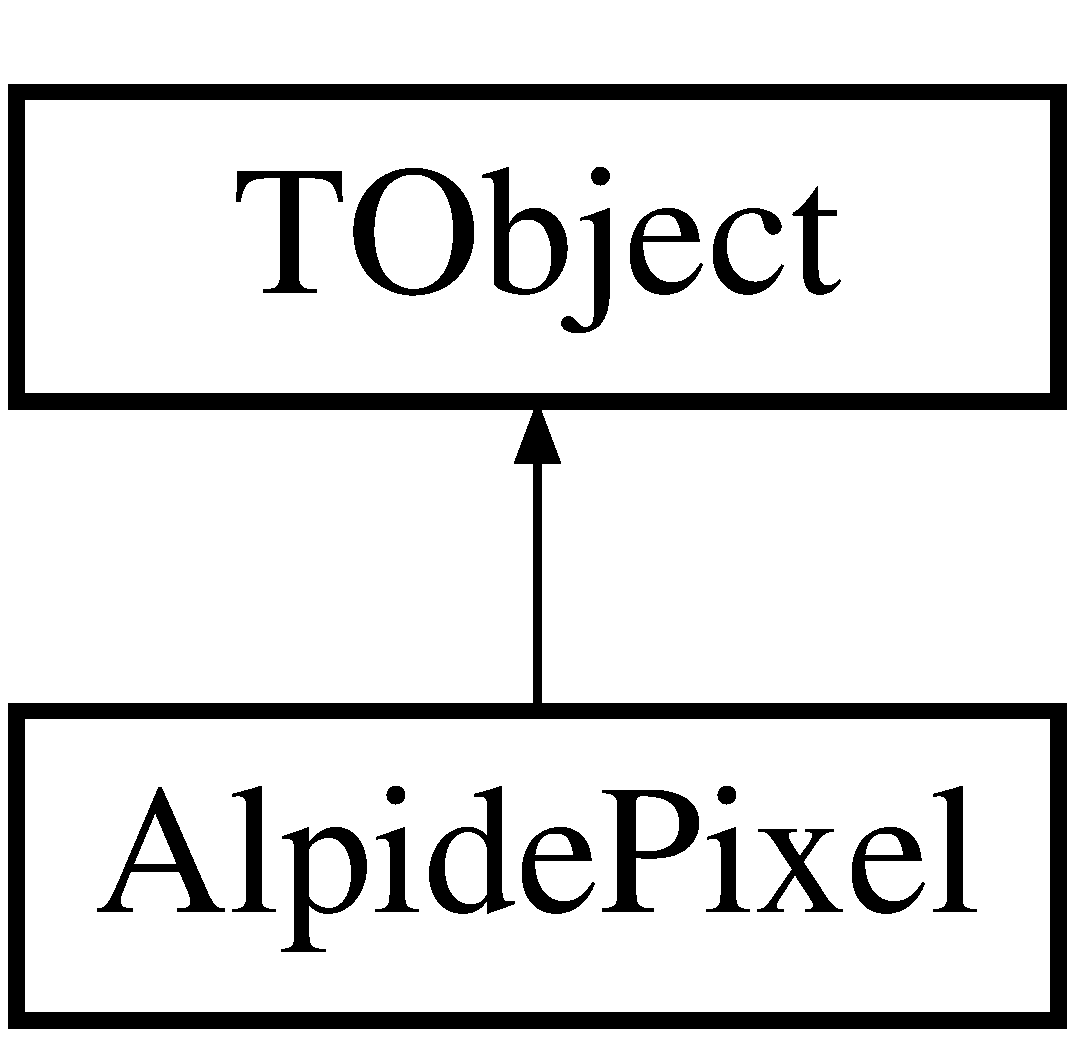
\includegraphics[height=2.000000cm]{class_alpide_pixel}
\end{center}
\end{figure}
\subsection*{Public Member Functions}
\begin{DoxyCompactItemize}
\item 
\mbox{\Hypertarget{class_alpide_pixel_a0ead4d3c0d6dd2039573584fdfadc58e}\label{class_alpide_pixel_a0ead4d3c0d6dd2039573584fdfadc58e}} 
{\bfseries Alpide\+Pixel} (Int\+\_\+t row, Int\+\_\+t col, Int\+\_\+t n\+Hits)
\item 
\mbox{\Hypertarget{class_alpide_pixel_a4169eb88465395230dd8771494bed982}\label{class_alpide_pixel_a4169eb88465395230dd8771494bed982}} 
Int\+\_\+t {\bfseries Get\+Col} () const
\item 
\mbox{\Hypertarget{class_alpide_pixel_acfa0e8e4238632f7395f1cf5d5870f87}\label{class_alpide_pixel_acfa0e8e4238632f7395f1cf5d5870f87}} 
Int\+\_\+t {\bfseries Get\+Row} () const
\item 
\mbox{\Hypertarget{class_alpide_pixel_a33c8d29096ed42e8ac5223106d850258}\label{class_alpide_pixel_a33c8d29096ed42e8ac5223106d850258}} 
Int\+\_\+t {\bfseries Get\+Number\+Of\+Hits} () const
\item 
\mbox{\Hypertarget{class_alpide_pixel_af034dd404d83563ea4432b65121c2ffb}\label{class_alpide_pixel_af034dd404d83563ea4432b65121c2ffb}} 
Double\+\_\+t {\bfseries Get\+X\+Coordinate} () const
\item 
\mbox{\Hypertarget{class_alpide_pixel_a9c0831870db24562a4cf3ffafa48f1ce}\label{class_alpide_pixel_a9c0831870db24562a4cf3ffafa48f1ce}} 
Double\+\_\+t {\bfseries Get\+Y\+Coordinate} () const
\item 
\mbox{\Hypertarget{class_alpide_pixel_ac58e1fa2fe45f8808728bfe08e83618f}\label{class_alpide_pixel_ac58e1fa2fe45f8808728bfe08e83618f}} 
void {\bfseries Set\+Col\+And\+Row} (Int\+\_\+t col, Int\+\_\+t row)
\item 
\mbox{\Hypertarget{class_alpide_pixel_a1d490d001379d939dd0564b135775178}\label{class_alpide_pixel_a1d490d001379d939dd0564b135775178}} 
void {\bfseries Set\+Col} (Int\+\_\+t col)
\item 
\mbox{\Hypertarget{class_alpide_pixel_a56759b535e206322d700e60796232e66}\label{class_alpide_pixel_a56759b535e206322d700e60796232e66}} 
void {\bfseries Set\+Row} (Int\+\_\+t row)
\item 
\mbox{\Hypertarget{class_alpide_pixel_aac8f5fd8c008acf7fe5a74a82e64d959}\label{class_alpide_pixel_aac8f5fd8c008acf7fe5a74a82e64d959}} 
void {\bfseries Set\+Number\+Of\+Hits} (Int\+\_\+t n\+Hits)
\item 
\mbox{\Hypertarget{class_alpide_pixel_a421d61832be201b8e428261d241b2112}\label{class_alpide_pixel_a421d61832be201b8e428261d241b2112}} 
void {\bfseries Set\+X\+AndY} (Double\+\_\+t x, Double\+\_\+t y)
\item 
\mbox{\Hypertarget{class_alpide_pixel_a14cff7f77ec17c0eb630d3af95bd6140}\label{class_alpide_pixel_a14cff7f77ec17c0eb630d3af95bd6140}} 
void {\bfseries SetX} (Double\+\_\+t x)
\item 
\mbox{\Hypertarget{class_alpide_pixel_a7230e4b812c3344789db2017c75f16ed}\label{class_alpide_pixel_a7230e4b812c3344789db2017c75f16ed}} 
void {\bfseries SetY} (Double\+\_\+t y)
\item 
Bool\+\_\+t \mbox{\hyperlink{class_alpide_pixel_a48184caa692d77f6c4ad70e25f18a69b}{Is\+Two\+Pixels\+Touched}} (\mbox{\hyperlink{class_alpide_pixel}{Alpide\+Pixel}} $\ast$pixel)
\item 
Bool\+\_\+t \mbox{\hyperlink{class_alpide_pixel_af532dfd2d03d8ad769b9f4ec12f5df1f}{Is\+Pixel\+Added\+To\+Cluster}} () const
\item 
\mbox{\Hypertarget{class_alpide_pixel_a2e78f8c88f7bc9c37e5646afd534ebf3}\label{class_alpide_pixel_a2e78f8c88f7bc9c37e5646afd534ebf3}} 
void {\bfseries Flag\+Pixel\+As\+Added\+To\+Cluster} ()
\item 
\mbox{\Hypertarget{class_alpide_pixel_a8d76bcc687374b3a462c533f747f061a}\label{class_alpide_pixel_a8d76bcc687374b3a462c533f747f061a}} 
void {\bfseries Reset} ()
\item 
\mbox{\Hypertarget{class_alpide_pixel_a78d2c1e3548287ce5c05668ba7dbec0f}\label{class_alpide_pixel_a78d2c1e3548287ce5c05668ba7dbec0f}} 
{\bfseries Class\+Def} (\mbox{\hyperlink{class_alpide_pixel}{Alpide\+Pixel}}, 1)
\end{DoxyCompactItemize}
\subsection*{Private Attributes}
\begin{DoxyCompactItemize}
\item 
\mbox{\Hypertarget{class_alpide_pixel_aa0e9d04eec9253f63ebe26882aa04e39}\label{class_alpide_pixel_aa0e9d04eec9253f63ebe26882aa04e39}} 
Int\+\_\+t {\bfseries f\+Row}
\item 
\mbox{\Hypertarget{class_alpide_pixel_a80151cc0e4cdf1fc1aa265d49df36fcc}\label{class_alpide_pixel_a80151cc0e4cdf1fc1aa265d49df36fcc}} 
Int\+\_\+t {\bfseries f\+Col}
\item 
\mbox{\Hypertarget{class_alpide_pixel_afae3655c40885515ec07cf70f4641f8c}\label{class_alpide_pixel_afae3655c40885515ec07cf70f4641f8c}} 
Int\+\_\+t {\bfseries f\+Number\+Of\+Hits}
\item 
Double\+\_\+t \mbox{\hyperlink{class_alpide_pixel_a10324596fb2e133158add1bb476a94fe}{f\+X\+Coordinate}}
\item 
Double\+\_\+t \mbox{\hyperlink{class_alpide_pixel_a603313fe11571d8db63a05c26711e691}{f\+Y\+Coordinate}}
\item 
Bool\+\_\+t \mbox{\hyperlink{class_alpide_pixel_aba15cede4c878ffeccb6ad389ac37088}{f\+Added\+To\+Cluster}}
\end{DoxyCompactItemize}


\subsection{Detailed Description}
A simple class for a pixel. A pixel is represented by its row and column in the single sensor (chip). Currently, a row is in the X direction while Col is in the Y direction. 

\subsection{Member Function Documentation}
\mbox{\Hypertarget{class_alpide_pixel_af532dfd2d03d8ad769b9f4ec12f5df1f}\label{class_alpide_pixel_af532dfd2d03d8ad769b9f4ec12f5df1f}} 
\index{Alpide\+Pixel@{Alpide\+Pixel}!Is\+Pixel\+Added\+To\+Cluster@{Is\+Pixel\+Added\+To\+Cluster}}
\index{Is\+Pixel\+Added\+To\+Cluster@{Is\+Pixel\+Added\+To\+Cluster}!Alpide\+Pixel@{Alpide\+Pixel}}
\subsubsection{\texorpdfstring{Is\+Pixel\+Added\+To\+Cluster()}{IsPixelAddedToCluster()}}
{\footnotesize\ttfamily Bool\+\_\+t Alpide\+Pixel\+::\+Is\+Pixel\+Added\+To\+Cluster (\begin{DoxyParamCaption}{ }\end{DoxyParamCaption}) const\hspace{0.3cm}{\ttfamily [inline]}}

Check if a pixel is already added to a cluster \mbox{\Hypertarget{class_alpide_pixel_a48184caa692d77f6c4ad70e25f18a69b}\label{class_alpide_pixel_a48184caa692d77f6c4ad70e25f18a69b}} 
\index{Alpide\+Pixel@{Alpide\+Pixel}!Is\+Two\+Pixels\+Touched@{Is\+Two\+Pixels\+Touched}}
\index{Is\+Two\+Pixels\+Touched@{Is\+Two\+Pixels\+Touched}!Alpide\+Pixel@{Alpide\+Pixel}}
\subsubsection{\texorpdfstring{Is\+Two\+Pixels\+Touched()}{IsTwoPixelsTouched()}}
{\footnotesize\ttfamily Bool\+\_\+t Alpide\+Pixel\+::\+Is\+Two\+Pixels\+Touched (\begin{DoxyParamCaption}\item[{\mbox{\hyperlink{class_alpide_pixel}{Alpide\+Pixel}} $\ast$}]{pixel }\end{DoxyParamCaption})}

Check if two pixels touch each other. A function used in the clustering. 

\subsection{Member Data Documentation}
\mbox{\Hypertarget{class_alpide_pixel_aba15cede4c878ffeccb6ad389ac37088}\label{class_alpide_pixel_aba15cede4c878ffeccb6ad389ac37088}} 
\index{Alpide\+Pixel@{Alpide\+Pixel}!f\+Added\+To\+Cluster@{f\+Added\+To\+Cluster}}
\index{f\+Added\+To\+Cluster@{f\+Added\+To\+Cluster}!Alpide\+Pixel@{Alpide\+Pixel}}
\subsubsection{\texorpdfstring{f\+Added\+To\+Cluster}{fAddedToCluster}}
{\footnotesize\ttfamily Bool\+\_\+t Alpide\+Pixel\+::f\+Added\+To\+Cluster\hspace{0.3cm}{\ttfamily [private]}}

This flag is used during the clustering, a pixel will not considerd anymore of it is already added to a cluster \mbox{\Hypertarget{class_alpide_pixel_a10324596fb2e133158add1bb476a94fe}\label{class_alpide_pixel_a10324596fb2e133158add1bb476a94fe}} 
\index{Alpide\+Pixel@{Alpide\+Pixel}!f\+X\+Coordinate@{f\+X\+Coordinate}}
\index{f\+X\+Coordinate@{f\+X\+Coordinate}!Alpide\+Pixel@{Alpide\+Pixel}}
\subsubsection{\texorpdfstring{f\+X\+Coordinate}{fXCoordinate}}
{\footnotesize\ttfamily Double\+\_\+t Alpide\+Pixel\+::f\+X\+Coordinate\hspace{0.3cm}{\ttfamily [private]}}

X coordinate of the pixel in the global coordinate system \mbox{\Hypertarget{class_alpide_pixel_a603313fe11571d8db63a05c26711e691}\label{class_alpide_pixel_a603313fe11571d8db63a05c26711e691}} 
\index{Alpide\+Pixel@{Alpide\+Pixel}!f\+Y\+Coordinate@{f\+Y\+Coordinate}}
\index{f\+Y\+Coordinate@{f\+Y\+Coordinate}!Alpide\+Pixel@{Alpide\+Pixel}}
\subsubsection{\texorpdfstring{f\+Y\+Coordinate}{fYCoordinate}}
{\footnotesize\ttfamily Double\+\_\+t Alpide\+Pixel\+::f\+Y\+Coordinate\hspace{0.3cm}{\ttfamily [private]}}

Y coordinate of the pixel in the global coordinate system 

The documentation for this class was generated from the following files\+:\begin{DoxyCompactItemize}
\item 
/\+Users/tarhini/\+Desktop/\+M\+F\+T/test\+Beam\+Analysis/my-\/\+M\+F\+T-\/\+Analysis/src/Alpide\+Pixel.\+hpp\item 
/\+Users/tarhini/\+Desktop/\+M\+F\+T/test\+Beam\+Analysis/my-\/\+M\+F\+T-\/\+Analysis/src/Alpide\+Pixel.\+cpp\end{DoxyCompactItemize}

\hypertarget{class_alpide_telescope}{}\section{Alpide\+Telescope Class Reference}
\label{class_alpide_telescope}\index{Alpide\+Telescope@{Alpide\+Telescope}}


{\ttfamily \#include $<$Alpide\+Telescope.\+hpp$>$}

Inheritance diagram for Alpide\+Telescope\+:\begin{figure}[H]
\begin{center}
\leavevmode
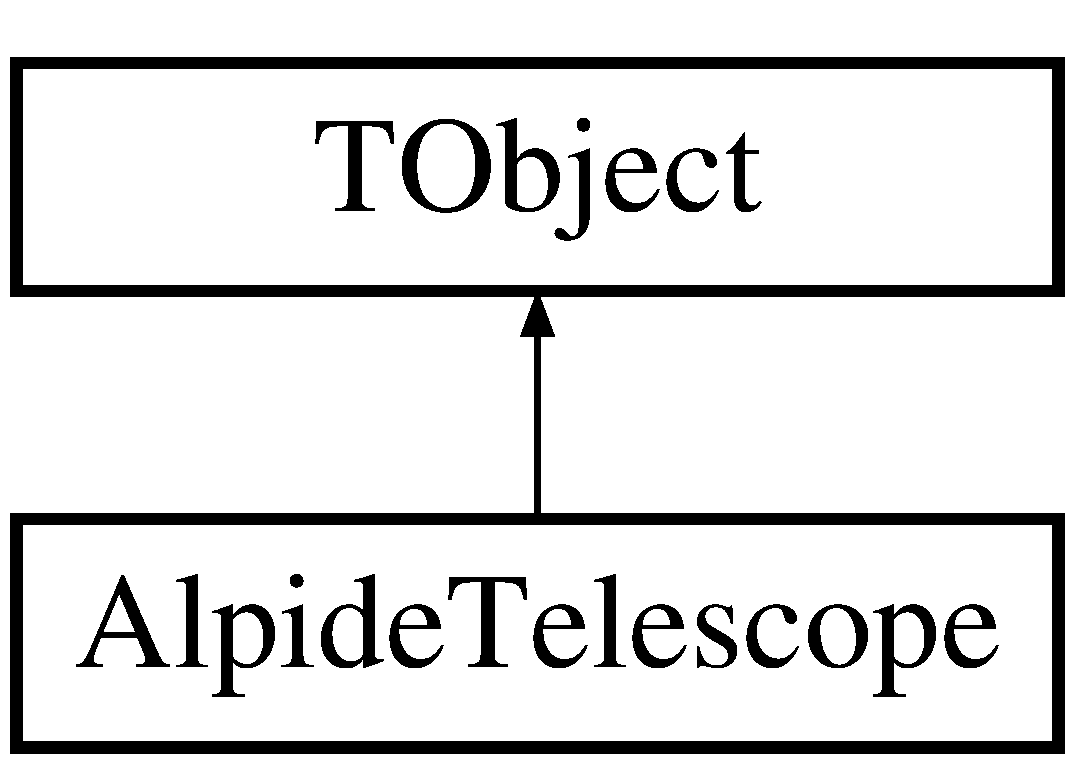
\includegraphics[height=2.000000cm]{class_alpide_telescope}
\end{center}
\end{figure}
\subsection*{Public Member Functions}
\begin{DoxyCompactItemize}
\item 
\mbox{\Hypertarget{class_alpide_telescope_a08b55fa73a002383c979d3cb4b6cf92b}\label{class_alpide_telescope_a08b55fa73a002383c979d3cb4b6cf92b}} 
Int\+\_\+t {\bfseries Get\+Telescope\+ID} () const
\item 
\mbox{\Hypertarget{class_alpide_telescope_ad08cbfeba32729bb79dece254fb76fd9}\label{class_alpide_telescope_ad08cbfeba32729bb79dece254fb76fd9}} 
Int\+\_\+t {\bfseries Get\+Number\+Of\+Chips} () const
\item 
\mbox{\Hypertarget{class_alpide_telescope_a619b34ba96df59daf0ddc85688138de5}\label{class_alpide_telescope_a619b34ba96df59daf0ddc85688138de5}} 
\mbox{\hyperlink{class_alpide_chip}{Alpide\+Chip}} $\ast$ {\bfseries Get\+Chip} (Int\+\_\+t index)
\item 
\mbox{\Hypertarget{class_alpide_telescope_af784289725c4f35046e7e9b9c72d6d2b}\label{class_alpide_telescope_af784289725c4f35046e7e9b9c72d6d2b}} 
\mbox{\hyperlink{class_alpide_chip}{Alpide\+Chip}} $\ast$ {\bfseries Get\+Chip\+By\+ID} (Int\+\_\+t chip\+ID)
\item 
\mbox{\Hypertarget{class_alpide_telescope_aa791e5afddf4cdd26ae5605856c3f6ce}\label{class_alpide_telescope_aa791e5afddf4cdd26ae5605856c3f6ce}} 
T\+Clones\+Array $\ast$ {\bfseries Get\+Array\+Chips} () const
\item 
\mbox{\Hypertarget{class_alpide_telescope_a7a6acb8b7a6dc6884ebeee2abd5183af}\label{class_alpide_telescope_a7a6acb8b7a6dc6884ebeee2abd5183af}} 
Int\+\_\+t {\bfseries Get\+Number\+Of\+Telescope\+Tracks} () const
\item 
\mbox{\Hypertarget{class_alpide_telescope_a4469548599474de64296350ee4619bfb}\label{class_alpide_telescope_a4469548599474de64296350ee4619bfb}} 
\mbox{\hyperlink{class_telescope_track}{Telescope\+Track}} $\ast$ {\bfseries Get\+Telescope\+Track} (Int\+\_\+t index)
\item 
\mbox{\Hypertarget{class_alpide_telescope_ad90f4b2850c1adaa40e87e1668ae6f6e}\label{class_alpide_telescope_ad90f4b2850c1adaa40e87e1668ae6f6e}} 
T\+Clones\+Array $\ast$ {\bfseries Get\+Array\+Telescope\+Tracks} () const
\item 
\mbox{\Hypertarget{class_alpide_telescope_a8369dd2fbb5e8ef0f33b5e4353986b16}\label{class_alpide_telescope_a8369dd2fbb5e8ef0f33b5e4353986b16}} 
void {\bfseries Set\+Telescope\+ID} (Int\+\_\+t telescope\+ID)
\item 
\mbox{\Hypertarget{class_alpide_telescope_a5c0d36c8e07025ea25e56daac3a5abe5}\label{class_alpide_telescope_a5c0d36c8e07025ea25e56daac3a5abe5}} 
void {\bfseries Add\+Chip} (\mbox{\hyperlink{class_alpide_chip}{Alpide\+Chip}} $\ast$chip)
\item 
\mbox{\Hypertarget{class_alpide_telescope_a7057a801f20d2178e09930298a18b3f7}\label{class_alpide_telescope_a7057a801f20d2178e09930298a18b3f7}} 
void {\bfseries Add\+Telescope\+Track} (\mbox{\hyperlink{class_telescope_track}{Telescope\+Track}} $\ast$track)
\item 
\mbox{\Hypertarget{class_alpide_telescope_a1fe138a228c478c7ec8f038b141ff29b}\label{class_alpide_telescope_a1fe138a228c478c7ec8f038b141ff29b}} 
void {\bfseries Reset\+Telescope} ()
\item 
\mbox{\Hypertarget{class_alpide_telescope_a0389541f27e727fe4f6cbd096d156e89}\label{class_alpide_telescope_a0389541f27e727fe4f6cbd096d156e89}} 
{\bfseries Class\+Def} (\mbox{\hyperlink{class_alpide_telescope}{Alpide\+Telescope}}, 1)
\end{DoxyCompactItemize}
\subsection*{Private Attributes}
\begin{DoxyCompactItemize}
\item 
Int\+\_\+t \mbox{\hyperlink{class_alpide_telescope_a9b885e9e99ae303294ba02f3bacd049b}{f\+Telescope\+ID}}
\item 
Int\+\_\+t \mbox{\hyperlink{class_alpide_telescope_ada9d09d4e2e419ab4c8da7a3da8f6395}{f\+Number\+Of\+Chips}}
\item 
T\+Clones\+Array $\ast$ \mbox{\hyperlink{class_alpide_telescope_aa660d33d3521ba7aa21930120e05e0cd}{f\+Array\+Chips}}
\item 
Int\+\_\+t \mbox{\hyperlink{class_alpide_telescope_a5767a235a504a73169601284b7f2f55c}{f\+Number\+Of\+Telescope\+Tracks}}
\item 
T\+Clones\+Array $\ast$ \mbox{\hyperlink{class_alpide_telescope_a98c999ffa985cf1161d8e17a0a1b2b0d}{f\+Array\+Telescope\+Tracks}}
\end{DoxyCompactItemize}


\subsection{Detailed Description}
A class for the alpide telescope. The telescope contains many (single?) alpide chips. It also contains an array of telescope tracks that will be added after fitting the cluster of its chips. T\+O\+DO\+: This class was developped before knowing that the telescope used in the test beam is also based on alpide chips, one cab think of making a detector class that can be either ladder or a telescope. 

\subsection{Member Data Documentation}
\mbox{\Hypertarget{class_alpide_telescope_aa660d33d3521ba7aa21930120e05e0cd}\label{class_alpide_telescope_aa660d33d3521ba7aa21930120e05e0cd}} 
\index{Alpide\+Telescope@{Alpide\+Telescope}!f\+Array\+Chips@{f\+Array\+Chips}}
\index{f\+Array\+Chips@{f\+Array\+Chips}!Alpide\+Telescope@{Alpide\+Telescope}}
\subsubsection{\texorpdfstring{f\+Array\+Chips}{fArrayChips}}
{\footnotesize\ttfamily T\+Clones\+Array$\ast$ Alpide\+Telescope\+::f\+Array\+Chips\hspace{0.3cm}{\ttfamily [private]}}

A vector of M\+T\+F\+Chips can be used but tobjarray may be more flexible in the further analysis. \mbox{\Hypertarget{class_alpide_telescope_a98c999ffa985cf1161d8e17a0a1b2b0d}\label{class_alpide_telescope_a98c999ffa985cf1161d8e17a0a1b2b0d}} 
\index{Alpide\+Telescope@{Alpide\+Telescope}!f\+Array\+Telescope\+Tracks@{f\+Array\+Telescope\+Tracks}}
\index{f\+Array\+Telescope\+Tracks@{f\+Array\+Telescope\+Tracks}!Alpide\+Telescope@{Alpide\+Telescope}}
\subsubsection{\texorpdfstring{f\+Array\+Telescope\+Tracks}{fArrayTelescopeTracks}}
{\footnotesize\ttfamily T\+Clones\+Array$\ast$ Alpide\+Telescope\+::f\+Array\+Telescope\+Tracks\hspace{0.3cm}{\ttfamily [private]}}

array of tracks from the telescope \mbox{\Hypertarget{class_alpide_telescope_ada9d09d4e2e419ab4c8da7a3da8f6395}\label{class_alpide_telescope_ada9d09d4e2e419ab4c8da7a3da8f6395}} 
\index{Alpide\+Telescope@{Alpide\+Telescope}!f\+Number\+Of\+Chips@{f\+Number\+Of\+Chips}}
\index{f\+Number\+Of\+Chips@{f\+Number\+Of\+Chips}!Alpide\+Telescope@{Alpide\+Telescope}}
\subsubsection{\texorpdfstring{f\+Number\+Of\+Chips}{fNumberOfChips}}
{\footnotesize\ttfamily Int\+\_\+t Alpide\+Telescope\+::f\+Number\+Of\+Chips\hspace{0.3cm}{\ttfamily [private]}}

number of chips in the telescope. \mbox{\Hypertarget{class_alpide_telescope_a5767a235a504a73169601284b7f2f55c}\label{class_alpide_telescope_a5767a235a504a73169601284b7f2f55c}} 
\index{Alpide\+Telescope@{Alpide\+Telescope}!f\+Number\+Of\+Telescope\+Tracks@{f\+Number\+Of\+Telescope\+Tracks}}
\index{f\+Number\+Of\+Telescope\+Tracks@{f\+Number\+Of\+Telescope\+Tracks}!Alpide\+Telescope@{Alpide\+Telescope}}
\subsubsection{\texorpdfstring{f\+Number\+Of\+Telescope\+Tracks}{fNumberOfTelescopeTracks}}
{\footnotesize\ttfamily Int\+\_\+t Alpide\+Telescope\+::f\+Number\+Of\+Telescope\+Tracks\hspace{0.3cm}{\ttfamily [private]}}

number of telescope tracks. (Do we expect one track per event or what ?) \mbox{\Hypertarget{class_alpide_telescope_a9b885e9e99ae303294ba02f3bacd049b}\label{class_alpide_telescope_a9b885e9e99ae303294ba02f3bacd049b}} 
\index{Alpide\+Telescope@{Alpide\+Telescope}!f\+Telescope\+ID@{f\+Telescope\+ID}}
\index{f\+Telescope\+ID@{f\+Telescope\+ID}!Alpide\+Telescope@{Alpide\+Telescope}}
\subsubsection{\texorpdfstring{f\+Telescope\+ID}{fTelescopeID}}
{\footnotesize\ttfamily Int\+\_\+t Alpide\+Telescope\+::f\+Telescope\+ID\hspace{0.3cm}{\ttfamily [private]}}

ID of the telescope as it appears in the raw file. 

The documentation for this class was generated from the following files\+:\begin{DoxyCompactItemize}
\item 
/\+Users/tarhini/\+Desktop/\+M\+F\+T/test\+Beam\+Analysis/my-\/\+M\+F\+T-\/\+Analysis/src/Alpide\+Telescope.\+hpp\item 
/\+Users/tarhini/\+Desktop/\+M\+F\+T/test\+Beam\+Analysis/my-\/\+M\+F\+T-\/\+Analysis/src/Alpide\+Telescope.\+cpp\end{DoxyCompactItemize}

\hypertarget{class_event_reader}{}\section{Event\+Reader Class Reference}
\label{class_event_reader}\index{Event\+Reader@{Event\+Reader}}


{\ttfamily \#include $<$Event\+Reader.\+hpp$>$}

Inheritance diagram for Event\+Reader\+:\begin{figure}[H]
\begin{center}
\leavevmode
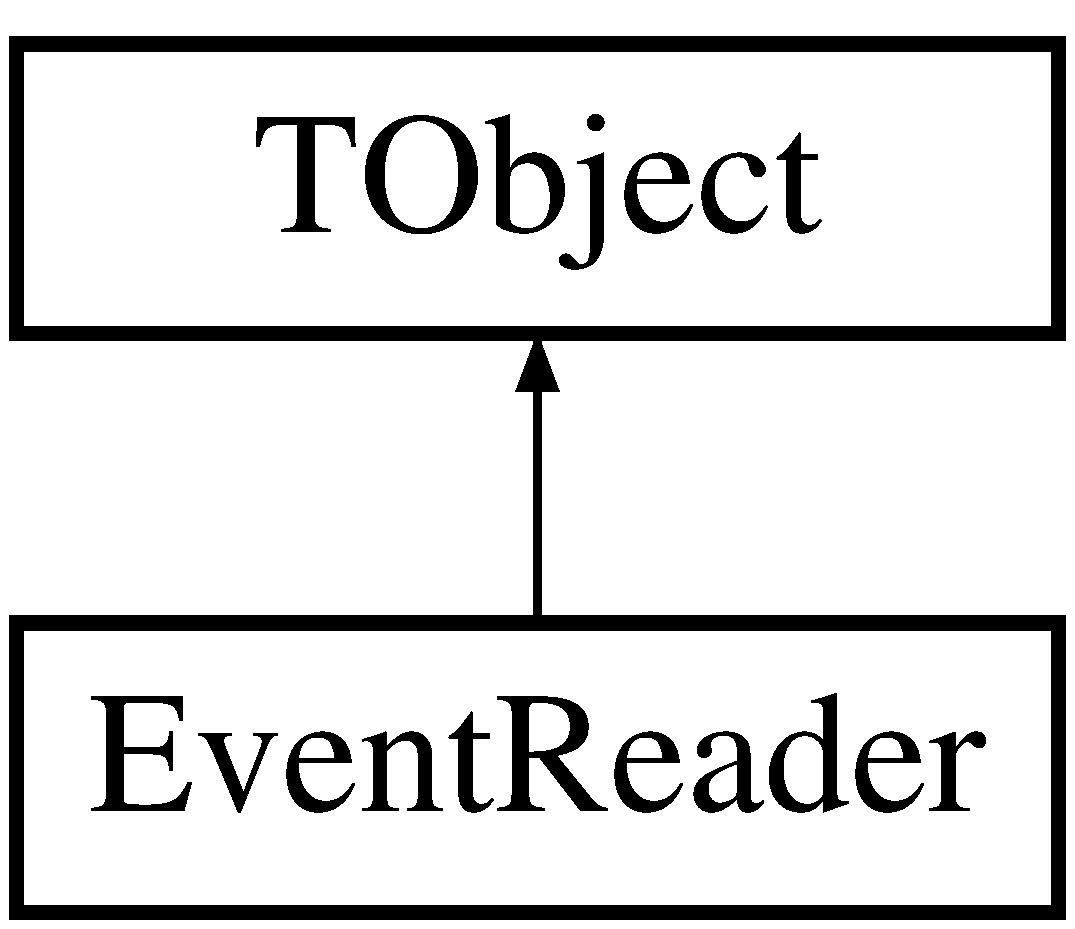
\includegraphics[height=2.000000cm]{class_event_reader}
\end{center}
\end{figure}
\subsection*{Public Member Functions}
\begin{DoxyCompactItemize}
\item 
\mbox{\Hypertarget{class_event_reader_a5cdb5f2917289e844712d36ac1b824d0}\label{class_event_reader_a5cdb5f2917289e844712d36ac1b824d0}} 
Bool\+\_\+t {\bfseries Set\+Input\+File} (const char $\ast$file\+Name)
\item 
\mbox{\Hypertarget{class_event_reader_a06bd8342adaa0f6c16582edfb9ea9db7}\label{class_event_reader_a06bd8342adaa0f6c16582edfb9ea9db7}} 
Bool\+\_\+t {\bfseries Read\+Event} ()
\item 
\mbox{\Hypertarget{class_event_reader_a5f403f1954a8d0efb384a5f680e011ee}\label{class_event_reader_a5f403f1954a8d0efb384a5f680e011ee}} 
Bool\+\_\+t {\bfseries Is\+Last\+Event} ()
\item 
\mbox{\Hypertarget{class_event_reader_afa588e79e61b7e2442e60501ec67872f}\label{class_event_reader_afa588e79e61b7e2442e60501ec67872f}} 
Int\+\_\+t {\bfseries Get\+Event\+Counter} ()
\item 
\mbox{\Hypertarget{class_event_reader_a70cdc9261406406bad39d1a767a931a2}\label{class_event_reader_a70cdc9261406406bad39d1a767a931a2}} 
Int\+\_\+t {\bfseries Get\+Number\+Of\+Hit\+Pixels} ()
\item 
\mbox{\Hypertarget{class_event_reader_ae34edd27c8906826a6483a49cfc6be4e}\label{class_event_reader_ae34edd27c8906826a6483a49cfc6be4e}} 
Bool\+\_\+t {\bfseries Get\+Next\+Hit\+Pixel} (Int\+\_\+t $\ast$array\+Detector\+ID, Int\+\_\+t $\ast$array\+Chip\+ID, Int\+\_\+t $\ast$array\+First\+Address, Int\+\_\+t $\ast$array\+Second\+Address, Int\+\_\+t $\ast$array\+N\+Hits)
\item 
\mbox{\Hypertarget{class_event_reader_a80faf6c115bb8f28e92efa7516a41bfc}\label{class_event_reader_a80faf6c115bb8f28e92efa7516a41bfc}} 
void {\bfseries Reset\+Hit\+Pixels\+Iter} ()
\item 
\mbox{\Hypertarget{class_event_reader_ad7c0063d0bea5faf1125c4e594e89b83}\label{class_event_reader_ad7c0063d0bea5faf1125c4e594e89b83}} 
Bool\+\_\+t {\bfseries Check\+Double\+Hit\+Pixels} (Bool\+\_\+t remove)
\end{DoxyCompactItemize}
\subsection*{Private Attributes}
\begin{DoxyCompactItemize}
\item 
ifstream \mbox{\hyperlink{class_event_reader_aaec259fd474a164d259caf942bbca0c4}{f\+Input\+File}}
\item 
Bool\+\_\+t \mbox{\hyperlink{class_event_reader_ae44339b541ef8d3e88cf5b3bb6d3e4a2}{f\+First\+Event}}
\item 
\mbox{\Hypertarget{class_event_reader_a55cc11a5908df56e887d7326fada22b3}\label{class_event_reader_a55cc11a5908df56e887d7326fada22b3}} 
Bool\+\_\+t {\bfseries f\+Last\+Event}
\item 
\mbox{\Hypertarget{class_event_reader_aef9c1e84a2c6a1c99aa29d249542f5a8}\label{class_event_reader_aef9c1e84a2c6a1c99aa29d249542f5a8}} 
Int\+\_\+t {\bfseries f\+Hit\+Pixels\+Iter}
\item 
Int\+\_\+t \mbox{\hyperlink{class_event_reader_a47a3228d169ec69259a5abb857ee0d0d}{f\+Event\+Counter}}
\item 
Int\+\_\+t \mbox{\hyperlink{class_event_reader_ac738aecc11ef01f0ced6d9de39701848}{f\+Current\+Event}}
\item 
\mbox{\Hypertarget{class_event_reader_aead189b9a419e811d32e89a61f9dd198}\label{class_event_reader_aead189b9a419e811d32e89a61f9dd198}} 
std\+::vector$<$ Int\+\_\+t $>$ {\bfseries f\+Vector\+Hit\+Pixels\+Detector\+ID}
\item 
\mbox{\Hypertarget{class_event_reader_a7f9506d70e35fedb27ba8717c81ef181}\label{class_event_reader_a7f9506d70e35fedb27ba8717c81ef181}} 
std\+::vector$<$ Int\+\_\+t $>$ {\bfseries f\+Vector\+Hit\+Pixels\+Chip\+ID}
\item 
\mbox{\Hypertarget{class_event_reader_a9b1246342dd793ef1b8bf436b1cf724e}\label{class_event_reader_a9b1246342dd793ef1b8bf436b1cf724e}} 
std\+::vector$<$ Int\+\_\+t $>$ {\bfseries f\+Vector\+Hit\+Pixels\+First\+Address}
\item 
\mbox{\Hypertarget{class_event_reader_a5fad84b4bd43b27c9499da8d749011f2}\label{class_event_reader_a5fad84b4bd43b27c9499da8d749011f2}} 
std\+::vector$<$ Int\+\_\+t $>$ {\bfseries f\+Vector\+Hit\+Pixels\+Second\+Address}
\item 
\mbox{\Hypertarget{class_event_reader_a08d796f609bff0725f0081a5646b5452}\label{class_event_reader_a08d796f609bff0725f0081a5646b5452}} 
std\+::vector$<$ Int\+\_\+t $>$ {\bfseries f\+Vector\+Hit\+Pixels\+N\+Hits}
\end{DoxyCompactItemize}


\subsection{Detailed Description}
This class handle the reading of the .txt (or .dat) file and so that the hit info can be stored. This class is obsolete for the analysis of real data since hits are now stored in a T\+Tree instead of .dat. This class however is needed to read generated files for tests purpose. 

\subsection{Member Data Documentation}
\mbox{\Hypertarget{class_event_reader_ac738aecc11ef01f0ced6d9de39701848}\label{class_event_reader_ac738aecc11ef01f0ced6d9de39701848}} 
\index{Event\+Reader@{Event\+Reader}!f\+Current\+Event@{f\+Current\+Event}}
\index{f\+Current\+Event@{f\+Current\+Event}!Event\+Reader@{Event\+Reader}}
\subsubsection{\texorpdfstring{f\+Current\+Event}{fCurrentEvent}}
{\footnotesize\ttfamily Int\+\_\+t Event\+Reader\+::f\+Current\+Event\hspace{0.3cm}{\ttfamily [private]}}

current event ID \mbox{\Hypertarget{class_event_reader_a47a3228d169ec69259a5abb857ee0d0d}\label{class_event_reader_a47a3228d169ec69259a5abb857ee0d0d}} 
\index{Event\+Reader@{Event\+Reader}!f\+Event\+Counter@{f\+Event\+Counter}}
\index{f\+Event\+Counter@{f\+Event\+Counter}!Event\+Reader@{Event\+Reader}}
\subsubsection{\texorpdfstring{f\+Event\+Counter}{fEventCounter}}
{\footnotesize\ttfamily Int\+\_\+t Event\+Reader\+::f\+Event\+Counter\hspace{0.3cm}{\ttfamily [private]}}

internal event counter (= event ID of next event) \mbox{\Hypertarget{class_event_reader_ae44339b541ef8d3e88cf5b3bb6d3e4a2}\label{class_event_reader_ae44339b541ef8d3e88cf5b3bb6d3e4a2}} 
\index{Event\+Reader@{Event\+Reader}!f\+First\+Event@{f\+First\+Event}}
\index{f\+First\+Event@{f\+First\+Event}!Event\+Reader@{Event\+Reader}}
\subsubsection{\texorpdfstring{f\+First\+Event}{fFirstEvent}}
{\footnotesize\ttfamily Bool\+\_\+t Event\+Reader\+::f\+First\+Event\hspace{0.3cm}{\ttfamily [private]}}

This is true when creating the event\+Reader object and is toogled to false when the first event is read. \mbox{\Hypertarget{class_event_reader_aaec259fd474a164d259caf942bbca0c4}\label{class_event_reader_aaec259fd474a164d259caf942bbca0c4}} 
\index{Event\+Reader@{Event\+Reader}!f\+Input\+File@{f\+Input\+File}}
\index{f\+Input\+File@{f\+Input\+File}!Event\+Reader@{Event\+Reader}}
\subsubsection{\texorpdfstring{f\+Input\+File}{fInputFile}}
{\footnotesize\ttfamily ifstream Event\+Reader\+::f\+Input\+File\hspace{0.3cm}{\ttfamily [private]}}

input text file. it can be .txt, or other extensions (e.\+g .dat) 

The documentation for this class was generated from the following files\+:\begin{DoxyCompactItemize}
\item 
/\+Users/tarhini/\+Desktop/\+M\+F\+T/test\+Beam\+Analysis/my-\/\+M\+F\+T-\/\+Analysis/src/Event\+Reader.\+hpp\item 
/\+Users/tarhini/\+Desktop/\+M\+F\+T/test\+Beam\+Analysis/my-\/\+M\+F\+T-\/\+Analysis/src/Event\+Reader.\+cpp\end{DoxyCompactItemize}

\hypertarget{struct_telescope_track_1_1_sum_distance2_object}{}\section{Telescope\+Track\+:\+:Sum\+Distance2\+Object Struct Reference}
\label{struct_telescope_track_1_1_sum_distance2_object}\index{Telescope\+Track\+::\+Sum\+Distance2\+Object@{Telescope\+Track\+::\+Sum\+Distance2\+Object}}
\subsection*{Public Member Functions}
\begin{DoxyCompactItemize}
\item 
\mbox{\Hypertarget{struct_telescope_track_1_1_sum_distance2_object_ae3ccb274f2191e028ce952179e9ec84c}\label{struct_telescope_track_1_1_sum_distance2_object_ae3ccb274f2191e028ce952179e9ec84c}} 
{\bfseries Sum\+Distance2\+Object} (T\+Graph2D $\ast$g)
\item 
\mbox{\Hypertarget{struct_telescope_track_1_1_sum_distance2_object_a916314f3e57da425cd578cec12b136c0}\label{struct_telescope_track_1_1_sum_distance2_object_a916314f3e57da425cd578cec12b136c0}} 
Double\+\_\+t {\bfseries Line\+Point\+Distance2} (Double\+\_\+t x, Double\+\_\+t y, Double\+\_\+t z, const Double\+\_\+t $\ast$line\+Params)
\item 
\mbox{\Hypertarget{struct_telescope_track_1_1_sum_distance2_object_af7634ef093c114cb7457cbea0445b52d}\label{struct_telescope_track_1_1_sum_distance2_object_af7634ef093c114cb7457cbea0445b52d}} 
double {\bfseries operator()} (const double $\ast$line\+Params)
\end{DoxyCompactItemize}
\subsection*{Public Attributes}
\begin{DoxyCompactItemize}
\item 
\mbox{\Hypertarget{struct_telescope_track_1_1_sum_distance2_object_aaa771260b176fef3365841e0b532ca15}\label{struct_telescope_track_1_1_sum_distance2_object_aaa771260b176fef3365841e0b532ca15}} 
T\+Graph2D $\ast$ {\bfseries line\+Graph}
\end{DoxyCompactItemize}


The documentation for this struct was generated from the following file\+:\begin{DoxyCompactItemize}
\item 
/\+Users/tarhini/\+Desktop/\+M\+F\+T/test\+Beam\+Analysis/my-\/\+M\+F\+T-\/\+Analysis/src/Telescope\+Track.\+hpp\end{DoxyCompactItemize}

\hypertarget{class_telescope_track}{}\section{Telescope\+Track Class Reference}
\label{class_telescope_track}\index{Telescope\+Track@{Telescope\+Track}}


{\ttfamily \#include $<$Telescope\+Track.\+hpp$>$}

Inheritance diagram for Telescope\+Track\+:\begin{figure}[H]
\begin{center}
\leavevmode
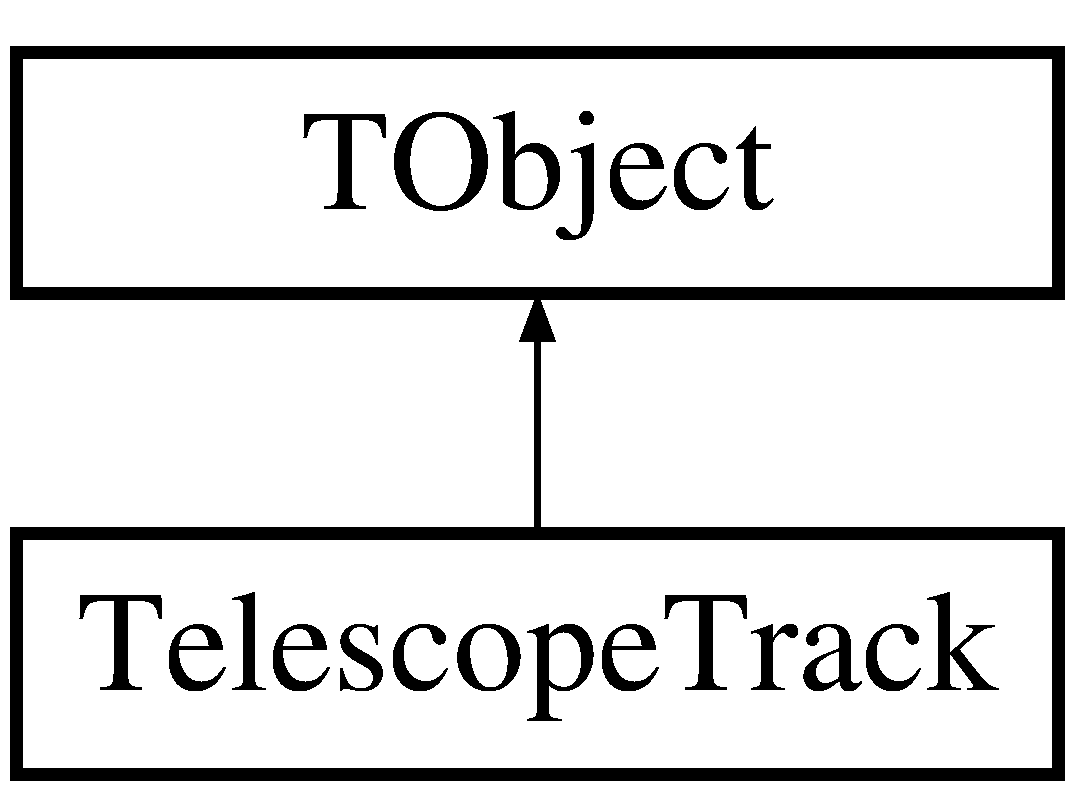
\includegraphics[height=2.000000cm]{class_telescope_track}
\end{center}
\end{figure}
\subsection*{Classes}
\begin{DoxyCompactItemize}
\item 
struct \mbox{\hyperlink{struct_telescope_track_1_1_sum_distance2_object}{Sum\+Distance2\+Object}}
\end{DoxyCompactItemize}
\subsection*{Public Member Functions}
\begin{DoxyCompactItemize}
\item 
\mbox{\Hypertarget{class_telescope_track_aa21071ed77d0b2bbf9d5bbc7b441afc4}\label{class_telescope_track_aa21071ed77d0b2bbf9d5bbc7b441afc4}} 
{\bfseries Telescope\+Track} (Int\+\_\+t track\+ID, Float\+\_\+t x\+Constant, Float\+\_\+t x\+Slope, Float\+\_\+t y\+Constant, Float\+\_\+t y\+Slope)
\item 
\mbox{\Hypertarget{class_telescope_track_af278076d355dd07da9ecea8a1807e099}\label{class_telescope_track_af278076d355dd07da9ecea8a1807e099}} 
Int\+\_\+t {\bfseries Get\+Track\+ID} ()
\item 
\mbox{\Hypertarget{class_telescope_track_a6d131c17d16f466db7d4a53209b47569}\label{class_telescope_track_a6d131c17d16f466db7d4a53209b47569}} 
Float\+\_\+t {\bfseries Get\+X\+Constant} () const
\item 
\mbox{\Hypertarget{class_telescope_track_ab4619449c0f1e1cdf1f52f37cc9d332f}\label{class_telescope_track_ab4619449c0f1e1cdf1f52f37cc9d332f}} 
Float\+\_\+t {\bfseries Get\+Y\+Constant} () const
\item 
\mbox{\Hypertarget{class_telescope_track_af3ca4b90a7261e3e1ed07d01bd51c7da}\label{class_telescope_track_af3ca4b90a7261e3e1ed07d01bd51c7da}} 
Float\+\_\+t {\bfseries Get\+X\+Slope} () const
\item 
\mbox{\Hypertarget{class_telescope_track_a3f150776a4329791920a795fb0ab0ac4}\label{class_telescope_track_a3f150776a4329791920a795fb0ab0ac4}} 
Float\+\_\+t {\bfseries Get\+Y\+Slope} () const
\item 
\mbox{\Hypertarget{class_telescope_track_ae0b86e4840ee2d648dd5e04dc69762d9}\label{class_telescope_track_ae0b86e4840ee2d648dd5e04dc69762d9}} 
Int\+\_\+t {\bfseries Get\+Number\+Of\+Points} () const
\item 
\mbox{\Hypertarget{class_telescope_track_a59f26eee73595a0f034d063cd1c13171}\label{class_telescope_track_a59f26eee73595a0f034d063cd1c13171}} 
std\+::vector$<$ Float\+\_\+t $>$ {\bfseries Get\+Vector\+PointsX} () const
\item 
\mbox{\Hypertarget{class_telescope_track_a52b7c3d8a0faf853465cbccbfc966447}\label{class_telescope_track_a52b7c3d8a0faf853465cbccbfc966447}} 
std\+::vector$<$ Float\+\_\+t $>$ {\bfseries Get\+Vector\+PointsY} () const
\item 
\mbox{\Hypertarget{class_telescope_track_a32ecf90e39c07c3efd0181d909b1c9d0}\label{class_telescope_track_a32ecf90e39c07c3efd0181d909b1c9d0}} 
std\+::vector$<$ Float\+\_\+t $>$ {\bfseries Get\+Vector\+PointsZ} () const
\item 
\mbox{\Hypertarget{class_telescope_track_a33d079747c4389c92b7e8136b0470ea6}\label{class_telescope_track_a33d079747c4389c92b7e8136b0470ea6}} 
Float\+\_\+t {\bfseries Get\+Chi\+Square} () const
\item 
void \mbox{\hyperlink{class_telescope_track_a6ab532f538116f6cdc97a4258b667d03}{Get\+X\+Y\+Coordinate}} (Float\+\_\+t \&x\+Coordinate, Float\+\_\+t \&y\+Coordinate, Float\+\_\+t z\+Coordiante)
\item 
\mbox{\Hypertarget{class_telescope_track_ab1956a4c99f2d2090fd3b7bcf8122254}\label{class_telescope_track_ab1956a4c99f2d2090fd3b7bcf8122254}} 
void {\bfseries Set\+Track\+ID} (Int\+\_\+t track\+ID)
\item 
\mbox{\Hypertarget{class_telescope_track_a251dd7613716b239ebfe7e2eda3f8ada}\label{class_telescope_track_a251dd7613716b239ebfe7e2eda3f8ada}} 
void {\bfseries Set\+ConstantX} (Float\+\_\+t x\+Constant)
\item 
\mbox{\Hypertarget{class_telescope_track_a4bdb85c9ea42c031b8eb575aae954ff0}\label{class_telescope_track_a4bdb85c9ea42c031b8eb575aae954ff0}} 
void {\bfseries Set\+ConstantY} (Float\+\_\+t y\+Constant)
\item 
\mbox{\Hypertarget{class_telescope_track_a89ac5a607b363654bc06abc7da8107a2}\label{class_telescope_track_a89ac5a607b363654bc06abc7da8107a2}} 
void {\bfseries Set\+SlopeX} (Float\+\_\+t x\+Slope)
\item 
\mbox{\Hypertarget{class_telescope_track_a9a05d679307b13d7a962312222085bbe}\label{class_telescope_track_a9a05d679307b13d7a962312222085bbe}} 
void {\bfseries Set\+SlopeY} (Float\+\_\+t y\+Slope)
\item 
\mbox{\Hypertarget{class_telescope_track_a9f4224a90fd4a19773513aab71b5e4e2}\label{class_telescope_track_a9f4224a90fd4a19773513aab71b5e4e2}} 
void {\bfseries Set\+Params} (Float\+\_\+t x\+Constant, Float\+\_\+t x\+Slope, Float\+\_\+t y\+Constant, Float\+\_\+t y\+Slope)
\item 
\mbox{\Hypertarget{class_telescope_track_aff1d178648c091a89af341ce24133355}\label{class_telescope_track_aff1d178648c091a89af341ce24133355}} 
void {\bfseries Set\+Chi\+Square} (Float\+\_\+t chi\+Square)
\item 
void \mbox{\hyperlink{class_telescope_track_afb3be5a992879f15abfb90906fd70856}{Add\+Point}} (Float\+\_\+t x, Float\+\_\+t y, Float\+\_\+t z)
\item 
\mbox{\Hypertarget{class_telescope_track_a449557b14b4f59237a14e425b8f35f03}\label{class_telescope_track_a449557b14b4f59237a14e425b8f35f03}} 
void {\bfseries Set\+Print\+Results} (Bool\+\_\+t b)
\item 
\mbox{\Hypertarget{class_telescope_track_ab4ea8add9de20aa04af48783d1514c91}\label{class_telescope_track_ab4ea8add9de20aa04af48783d1514c91}} 
void {\bfseries Reset} ()
\item 
\mbox{\Hypertarget{class_telescope_track_a1eb2b141f7ed1063fa901ed00cf8b90e}\label{class_telescope_track_a1eb2b141f7ed1063fa901ed00cf8b90e}} 
void {\bfseries Fit\+Track} ()
\item 
\mbox{\Hypertarget{class_telescope_track_aa041988968d0ed95afd593011bccfa9f}\label{class_telescope_track_aa041988968d0ed95afd593011bccfa9f}} 
{\bfseries Class\+Def} (\mbox{\hyperlink{class_telescope_track}{Telescope\+Track}}, 1)
\end{DoxyCompactItemize}
\subsection*{Private Attributes}
\begin{DoxyCompactItemize}
\item 
Int\+\_\+t \mbox{\hyperlink{class_telescope_track_a64977c9f478eba9beb2ae6026e0b7e0a}{f\+Track\+ID}}
\item 
Float\+\_\+t \mbox{\hyperlink{class_telescope_track_a3bab476931d460ea80cd9700c29ee2f9}{f\+X\+Constant}}
\item 
Float\+\_\+t \mbox{\hyperlink{class_telescope_track_a14fdd27ed94d2b69730e56fd2fbbc0ef}{f\+X\+Slope}}
\item 
Float\+\_\+t \mbox{\hyperlink{class_telescope_track_a8e5aa9428a73c38ce626d89bad494ec1}{f\+Y\+Constant}}
\item 
Float\+\_\+t \mbox{\hyperlink{class_telescope_track_aa522f83a156341cd06a868c9f4692953}{f\+Y\+Slope}}
\item 
\mbox{\Hypertarget{class_telescope_track_a5765f94c6ca2e1ca5c7074c20c410698}\label{class_telescope_track_a5765f94c6ca2e1ca5c7074c20c410698}} 
Int\+\_\+t {\bfseries f\+Number\+Of\+Points}
\item 
std\+::vector$<$ Float\+\_\+t $>$ \mbox{\hyperlink{class_telescope_track_a587fff80c330ef66a47017c0e0fe64e0}{f\+Vector\+PointsX}}
\item 
std\+::vector$<$ Float\+\_\+t $>$ \mbox{\hyperlink{class_telescope_track_ad299ce3251a1c5628bc3949effffe125}{f\+Vector\+PointsY}}
\item 
std\+::vector$<$ Float\+\_\+t $>$ \mbox{\hyperlink{class_telescope_track_ac1df4135d9b6d03c66397a017003c675}{f\+Vector\+PointsZ}}
\item 
Bool\+\_\+t \mbox{\hyperlink{class_telescope_track_ad7ef1d1faa561a6921cd1442d8856e64}{f\+Print\+Results}}
\item 
Float\+\_\+t \mbox{\hyperlink{class_telescope_track_a0254ea60690e1f619a64191b1ae1e726}{f\+Chi\+Square}}
\end{DoxyCompactItemize}


\subsection{Detailed Description}
A class for a telescope track. In the current implementation, the track is simply a staright line in 3d space with four parameters (constant and slope for X and Y). The line equation is\+: \{x = A + B$\ast$t\},\{y = C + D$\ast$t\}, \{z=t\} T\+O\+DO\+: Make this class more general (maybe use directly the T\+Track from root). 

\subsection{Member Function Documentation}
\mbox{\Hypertarget{class_telescope_track_afb3be5a992879f15abfb90906fd70856}\label{class_telescope_track_afb3be5a992879f15abfb90906fd70856}} 
\index{Telescope\+Track@{Telescope\+Track}!Add\+Point@{Add\+Point}}
\index{Add\+Point@{Add\+Point}!Telescope\+Track@{Telescope\+Track}}
\subsubsection{\texorpdfstring{Add\+Point()}{AddPoint()}}
{\footnotesize\ttfamily void Telescope\+Track\+::\+Add\+Point (\begin{DoxyParamCaption}\item[{Float\+\_\+t}]{x,  }\item[{Float\+\_\+t}]{y,  }\item[{Float\+\_\+t}]{z }\end{DoxyParamCaption})}

Add a point to the ensemble of points to be fitted \mbox{\Hypertarget{class_telescope_track_a6ab532f538116f6cdc97a4258b667d03}\label{class_telescope_track_a6ab532f538116f6cdc97a4258b667d03}} 
\index{Telescope\+Track@{Telescope\+Track}!Get\+X\+Y\+Coordinate@{Get\+X\+Y\+Coordinate}}
\index{Get\+X\+Y\+Coordinate@{Get\+X\+Y\+Coordinate}!Telescope\+Track@{Telescope\+Track}}
\subsubsection{\texorpdfstring{Get\+X\+Y\+Coordinate()}{GetXYCoordinate()}}
{\footnotesize\ttfamily void Telescope\+Track\+::\+Get\+X\+Y\+Coordinate (\begin{DoxyParamCaption}\item[{Float\+\_\+t \&}]{x\+Coordinate,  }\item[{Float\+\_\+t \&}]{y\+Coordinate,  }\item[{Float\+\_\+t}]{z\+Coordiante }\end{DoxyParamCaption})}

A function to get the X,Y coordinate for a given Z coordinate using the line equation. 

\subsection{Member Data Documentation}
\mbox{\Hypertarget{class_telescope_track_a0254ea60690e1f619a64191b1ae1e726}\label{class_telescope_track_a0254ea60690e1f619a64191b1ae1e726}} 
\index{Telescope\+Track@{Telescope\+Track}!f\+Chi\+Square@{f\+Chi\+Square}}
\index{f\+Chi\+Square@{f\+Chi\+Square}!Telescope\+Track@{Telescope\+Track}}
\subsubsection{\texorpdfstring{f\+Chi\+Square}{fChiSquare}}
{\footnotesize\ttfamily Float\+\_\+t Telescope\+Track\+::f\+Chi\+Square\hspace{0.3cm}{\ttfamily [private]}}

The track will be fitted using the hits in the telescope. A chisquare cut shall be applied to accept the tracks. \mbox{\Hypertarget{class_telescope_track_ad7ef1d1faa561a6921cd1442d8856e64}\label{class_telescope_track_ad7ef1d1faa561a6921cd1442d8856e64}} 
\index{Telescope\+Track@{Telescope\+Track}!f\+Print\+Results@{f\+Print\+Results}}
\index{f\+Print\+Results@{f\+Print\+Results}!Telescope\+Track@{Telescope\+Track}}
\subsubsection{\texorpdfstring{f\+Print\+Results}{fPrintResults}}
{\footnotesize\ttfamily Bool\+\_\+t Telescope\+Track\+::f\+Print\+Results\hspace{0.3cm}{\ttfamily [private]}}

Flag for printing results of the fit. Put to true when testing \mbox{\Hypertarget{class_telescope_track_a64977c9f478eba9beb2ae6026e0b7e0a}\label{class_telescope_track_a64977c9f478eba9beb2ae6026e0b7e0a}} 
\index{Telescope\+Track@{Telescope\+Track}!f\+Track\+ID@{f\+Track\+ID}}
\index{f\+Track\+ID@{f\+Track\+ID}!Telescope\+Track@{Telescope\+Track}}
\subsubsection{\texorpdfstring{f\+Track\+ID}{fTrackID}}
{\footnotesize\ttfamily Int\+\_\+t Telescope\+Track\+::f\+Track\+ID\hspace{0.3cm}{\ttfamily [private]}}

a track ID. Not used so far since in the evnt the track is identified by its index in the array. \mbox{\Hypertarget{class_telescope_track_a587fff80c330ef66a47017c0e0fe64e0}\label{class_telescope_track_a587fff80c330ef66a47017c0e0fe64e0}} 
\index{Telescope\+Track@{Telescope\+Track}!f\+Vector\+PointsX@{f\+Vector\+PointsX}}
\index{f\+Vector\+PointsX@{f\+Vector\+PointsX}!Telescope\+Track@{Telescope\+Track}}
\subsubsection{\texorpdfstring{f\+Vector\+PointsX}{fVectorPointsX}}
{\footnotesize\ttfamily std\+::vector$<$Float\+\_\+t$>$ Telescope\+Track\+::f\+Vector\+PointsX\hspace{0.3cm}{\ttfamily [private]}}

The x coordinates of the points added to the track fit \mbox{\Hypertarget{class_telescope_track_ad299ce3251a1c5628bc3949effffe125}\label{class_telescope_track_ad299ce3251a1c5628bc3949effffe125}} 
\index{Telescope\+Track@{Telescope\+Track}!f\+Vector\+PointsY@{f\+Vector\+PointsY}}
\index{f\+Vector\+PointsY@{f\+Vector\+PointsY}!Telescope\+Track@{Telescope\+Track}}
\subsubsection{\texorpdfstring{f\+Vector\+PointsY}{fVectorPointsY}}
{\footnotesize\ttfamily std\+::vector$<$Float\+\_\+t$>$ Telescope\+Track\+::f\+Vector\+PointsY\hspace{0.3cm}{\ttfamily [private]}}

The y coordinates of the points added to the track fit \mbox{\Hypertarget{class_telescope_track_ac1df4135d9b6d03c66397a017003c675}\label{class_telescope_track_ac1df4135d9b6d03c66397a017003c675}} 
\index{Telescope\+Track@{Telescope\+Track}!f\+Vector\+PointsZ@{f\+Vector\+PointsZ}}
\index{f\+Vector\+PointsZ@{f\+Vector\+PointsZ}!Telescope\+Track@{Telescope\+Track}}
\subsubsection{\texorpdfstring{f\+Vector\+PointsZ}{fVectorPointsZ}}
{\footnotesize\ttfamily std\+::vector$<$Float\+\_\+t$>$ Telescope\+Track\+::f\+Vector\+PointsZ\hspace{0.3cm}{\ttfamily [private]}}

The z coordinates of the points added to the track fit \mbox{\Hypertarget{class_telescope_track_a3bab476931d460ea80cd9700c29ee2f9}\label{class_telescope_track_a3bab476931d460ea80cd9700c29ee2f9}} 
\index{Telescope\+Track@{Telescope\+Track}!f\+X\+Constant@{f\+X\+Constant}}
\index{f\+X\+Constant@{f\+X\+Constant}!Telescope\+Track@{Telescope\+Track}}
\subsubsection{\texorpdfstring{f\+X\+Constant}{fXConstant}}
{\footnotesize\ttfamily Float\+\_\+t Telescope\+Track\+::f\+X\+Constant\hspace{0.3cm}{\ttfamily [private]}}

A in the above line equation \mbox{\Hypertarget{class_telescope_track_a14fdd27ed94d2b69730e56fd2fbbc0ef}\label{class_telescope_track_a14fdd27ed94d2b69730e56fd2fbbc0ef}} 
\index{Telescope\+Track@{Telescope\+Track}!f\+X\+Slope@{f\+X\+Slope}}
\index{f\+X\+Slope@{f\+X\+Slope}!Telescope\+Track@{Telescope\+Track}}
\subsubsection{\texorpdfstring{f\+X\+Slope}{fXSlope}}
{\footnotesize\ttfamily Float\+\_\+t Telescope\+Track\+::f\+X\+Slope\hspace{0.3cm}{\ttfamily [private]}}

B in the above line equation \mbox{\Hypertarget{class_telescope_track_a8e5aa9428a73c38ce626d89bad494ec1}\label{class_telescope_track_a8e5aa9428a73c38ce626d89bad494ec1}} 
\index{Telescope\+Track@{Telescope\+Track}!f\+Y\+Constant@{f\+Y\+Constant}}
\index{f\+Y\+Constant@{f\+Y\+Constant}!Telescope\+Track@{Telescope\+Track}}
\subsubsection{\texorpdfstring{f\+Y\+Constant}{fYConstant}}
{\footnotesize\ttfamily Float\+\_\+t Telescope\+Track\+::f\+Y\+Constant\hspace{0.3cm}{\ttfamily [private]}}

C in the above line equation \mbox{\Hypertarget{class_telescope_track_aa522f83a156341cd06a868c9f4692953}\label{class_telescope_track_aa522f83a156341cd06a868c9f4692953}} 
\index{Telescope\+Track@{Telescope\+Track}!f\+Y\+Slope@{f\+Y\+Slope}}
\index{f\+Y\+Slope@{f\+Y\+Slope}!Telescope\+Track@{Telescope\+Track}}
\subsubsection{\texorpdfstring{f\+Y\+Slope}{fYSlope}}
{\footnotesize\ttfamily Float\+\_\+t Telescope\+Track\+::f\+Y\+Slope\hspace{0.3cm}{\ttfamily [private]}}

D in the above line equation 

The documentation for this class was generated from the following files\+:\begin{DoxyCompactItemize}
\item 
/\+Users/tarhini/\+Desktop/\+M\+F\+T/test\+Beam\+Analysis/my-\/\+M\+F\+T-\/\+Analysis/src/Telescope\+Track.\+hpp\item 
/\+Users/tarhini/\+Desktop/\+M\+F\+T/test\+Beam\+Analysis/my-\/\+M\+F\+T-\/\+Analysis/src/Telescope\+Track.\+cpp\end{DoxyCompactItemize}

\hypertarget{class_test_beam_event}{}\section{Test\+Beam\+Event Class Reference}
\label{class_test_beam_event}\index{Test\+Beam\+Event@{Test\+Beam\+Event}}


{\ttfamily \#include $<$Test\+Beam\+Event.\+hpp$>$}

Inheritance diagram for Test\+Beam\+Event\+:\begin{figure}[H]
\begin{center}
\leavevmode
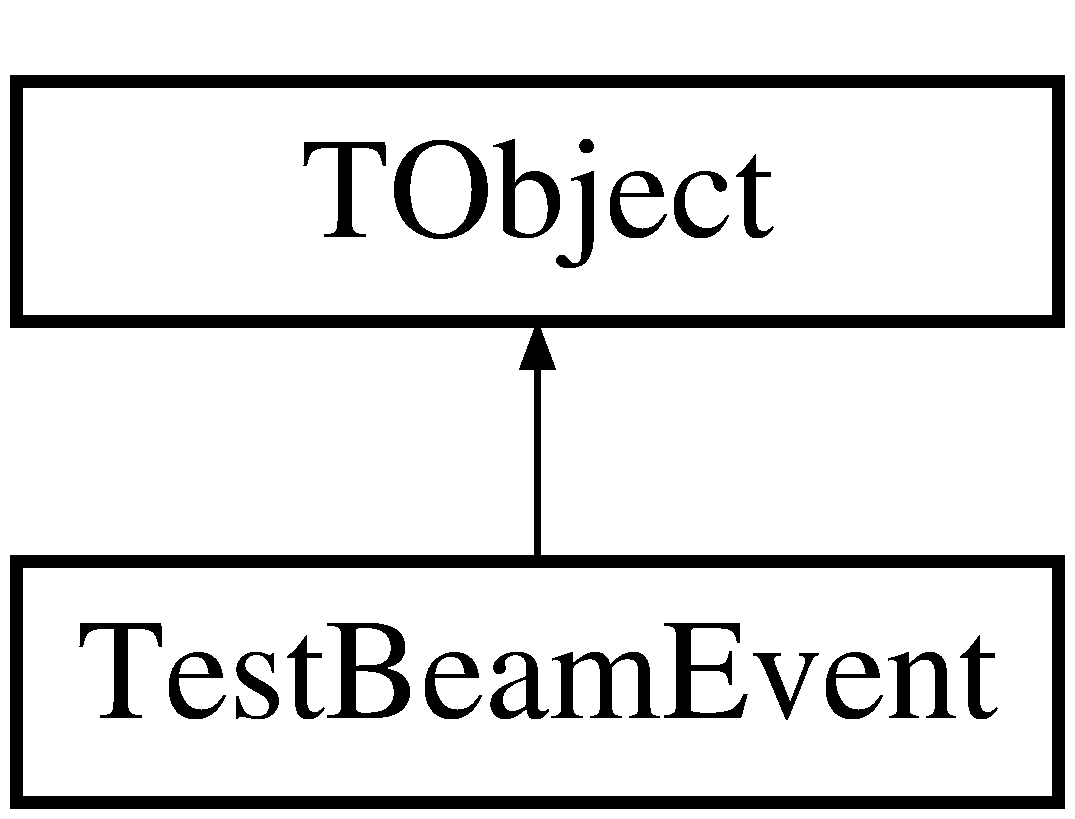
\includegraphics[height=2.000000cm]{class_test_beam_event}
\end{center}
\end{figure}
\subsection*{Public Member Functions}
\begin{DoxyCompactItemize}
\item 
\mbox{\Hypertarget{class_test_beam_event_a6eb03eb6d756ef2333730a7c45c384ff}\label{class_test_beam_event_a6eb03eb6d756ef2333730a7c45c384ff}} 
{\bfseries Test\+Beam\+Event} (int event\+ID)
\item 
\mbox{\Hypertarget{class_test_beam_event_a24181fa9039970765268659c88c1f514}\label{class_test_beam_event_a24181fa9039970765268659c88c1f514}} 
Int\+\_\+t {\bfseries Get\+Event\+ID} () const
\item 
\mbox{\Hypertarget{class_test_beam_event_a2bf15ab9482d7fd02436487baba2efe5}\label{class_test_beam_event_a2bf15ab9482d7fd02436487baba2efe5}} 
Int\+\_\+t {\bfseries Get\+Number\+Of\+Ladders} () const
\item 
\mbox{\Hypertarget{class_test_beam_event_af0ec87e7f48f72e0e862dffc53815db5}\label{class_test_beam_event_af0ec87e7f48f72e0e862dffc53815db5}} 
\mbox{\hyperlink{class_alpide_telescope}{Alpide\+Telescope}} $\ast$ {\bfseries Get\+Telescope} () const
\item 
\mbox{\Hypertarget{class_test_beam_event_ab39a199bb41a78b8a5d8d0ae564c9294}\label{class_test_beam_event_ab39a199bb41a78b8a5d8d0ae564c9294}} 
\mbox{\hyperlink{class_alpide_ladder}{Alpide\+Ladder}} $\ast$ {\bfseries Get\+Ladder} (Int\+\_\+t index)
\item 
\mbox{\Hypertarget{class_test_beam_event_a0c24b61aa21b532fb9b75e9a6174b8ab}\label{class_test_beam_event_a0c24b61aa21b532fb9b75e9a6174b8ab}} 
\mbox{\hyperlink{class_alpide_ladder}{Alpide\+Ladder}} $\ast$ {\bfseries Get\+Ladder\+By\+Id} (Int\+\_\+t ladder\+ID)
\item 
\mbox{\Hypertarget{class_test_beam_event_a42227b3585f6168c4fe20fc3743d2853}\label{class_test_beam_event_a42227b3585f6168c4fe20fc3743d2853}} 
T\+Clones\+Array $\ast$ {\bfseries Get\+Array\+Ladders} () const
\item 
\mbox{\Hypertarget{class_test_beam_event_afd3a06a34d7c2ad20c18540055704f89}\label{class_test_beam_event_afd3a06a34d7c2ad20c18540055704f89}} 
void {\bfseries Add\+Ladder} (\mbox{\hyperlink{class_alpide_ladder}{Alpide\+Ladder}} $\ast$ladder)
\item 
\mbox{\Hypertarget{class_test_beam_event_a12430bdd449a4acb6c01a94729d5c774}\label{class_test_beam_event_a12430bdd449a4acb6c01a94729d5c774}} 
void {\bfseries Set\+Event\+ID} (Int\+\_\+t event\+ID)
\item 
\mbox{\Hypertarget{class_test_beam_event_a984f80797e7e21291c5259013e6d15f0}\label{class_test_beam_event_a984f80797e7e21291c5259013e6d15f0}} 
void {\bfseries Set\+Telescope} (\mbox{\hyperlink{class_alpide_telescope}{Alpide\+Telescope}} $\ast$telescope)
\item 
\mbox{\Hypertarget{class_test_beam_event_a8f69ed0160b21ddb51aeac4f1c8f362e}\label{class_test_beam_event_a8f69ed0160b21ddb51aeac4f1c8f362e}} 
void {\bfseries Reset\+Event} ()
\item 
\mbox{\Hypertarget{class_test_beam_event_a3d25446f0ca8fb7a11a69d0084e5fdfc}\label{class_test_beam_event_a3d25446f0ca8fb7a11a69d0084e5fdfc}} 
{\bfseries Class\+Def} (\mbox{\hyperlink{class_test_beam_event}{Test\+Beam\+Event}}, 1)
\end{DoxyCompactItemize}
\subsection*{Private Attributes}
\begin{DoxyCompactItemize}
\item 
Int\+\_\+t \mbox{\hyperlink{class_test_beam_event_a1282488fec26d6b83901407e75378dda}{f\+Event\+ID}}
\item 
Int\+\_\+t \mbox{\hyperlink{class_test_beam_event_aca631326d6c05616a55cc16349c8b339}{f\+Number\+Of\+Ladders}}
\item 
T\+Clones\+Array $\ast$ \mbox{\hyperlink{class_test_beam_event_ae24662632a14f052415b9b7eb76e31d6}{f\+Array\+Ladders}}
\item 
\mbox{\hyperlink{class_alpide_telescope}{Alpide\+Telescope}} $\ast$ \mbox{\hyperlink{class_test_beam_event_ade24f88970804477d66d35d6e5acfb98}{f\+Telescope}}
\end{DoxyCompactItemize}


\subsection{Detailed Description}
A class for an event of M\+FT test beam. An event has an id, an array of ladders, and a telescope. 

\subsection{Member Data Documentation}
\mbox{\Hypertarget{class_test_beam_event_ae24662632a14f052415b9b7eb76e31d6}\label{class_test_beam_event_ae24662632a14f052415b9b7eb76e31d6}} 
\index{Test\+Beam\+Event@{Test\+Beam\+Event}!f\+Array\+Ladders@{f\+Array\+Ladders}}
\index{f\+Array\+Ladders@{f\+Array\+Ladders}!Test\+Beam\+Event@{Test\+Beam\+Event}}
\subsubsection{\texorpdfstring{f\+Array\+Ladders}{fArrayLadders}}
{\footnotesize\ttfamily T\+Clones\+Array$\ast$ Test\+Beam\+Event\+::f\+Array\+Ladders\hspace{0.3cm}{\ttfamily [private]}}

A vector of Alpide\+Ladders can be used but tobjarray may be more flexible in the further analysis. \mbox{\Hypertarget{class_test_beam_event_a1282488fec26d6b83901407e75378dda}\label{class_test_beam_event_a1282488fec26d6b83901407e75378dda}} 
\index{Test\+Beam\+Event@{Test\+Beam\+Event}!f\+Event\+ID@{f\+Event\+ID}}
\index{f\+Event\+ID@{f\+Event\+ID}!Test\+Beam\+Event@{Test\+Beam\+Event}}
\subsubsection{\texorpdfstring{f\+Event\+ID}{fEventID}}
{\footnotesize\ttfamily Int\+\_\+t Test\+Beam\+Event\+::f\+Event\+ID\hspace{0.3cm}{\ttfamily [private]}}

event ID number \mbox{\Hypertarget{class_test_beam_event_aca631326d6c05616a55cc16349c8b339}\label{class_test_beam_event_aca631326d6c05616a55cc16349c8b339}} 
\index{Test\+Beam\+Event@{Test\+Beam\+Event}!f\+Number\+Of\+Ladders@{f\+Number\+Of\+Ladders}}
\index{f\+Number\+Of\+Ladders@{f\+Number\+Of\+Ladders}!Test\+Beam\+Event@{Test\+Beam\+Event}}
\subsubsection{\texorpdfstring{f\+Number\+Of\+Ladders}{fNumberOfLadders}}
{\footnotesize\ttfamily Int\+\_\+t Test\+Beam\+Event\+::f\+Number\+Of\+Ladders\hspace{0.3cm}{\ttfamily [private]}}

number of ladders in the event. Probably this will be common for all the events. \mbox{\Hypertarget{class_test_beam_event_ade24f88970804477d66d35d6e5acfb98}\label{class_test_beam_event_ade24f88970804477d66d35d6e5acfb98}} 
\index{Test\+Beam\+Event@{Test\+Beam\+Event}!f\+Telescope@{f\+Telescope}}
\index{f\+Telescope@{f\+Telescope}!Test\+Beam\+Event@{Test\+Beam\+Event}}
\subsubsection{\texorpdfstring{f\+Telescope}{fTelescope}}
{\footnotesize\ttfamily \mbox{\hyperlink{class_alpide_telescope}{Alpide\+Telescope}}$\ast$ Test\+Beam\+Event\+::f\+Telescope\hspace{0.3cm}{\ttfamily [private]}}

A class member where the telescope tracks and chips are stored. Only w-\/one telescope is supposed to be in the setup 

The documentation for this class was generated from the following files\+:\begin{DoxyCompactItemize}
\item 
/\+Users/tarhini/\+Desktop/\+M\+F\+T/test\+Beam\+Analysis/my-\/\+M\+F\+T-\/\+Analysis/src/Test\+Beam\+Event.\+hpp\item 
/\+Users/tarhini/\+Desktop/\+M\+F\+T/test\+Beam\+Analysis/my-\/\+M\+F\+T-\/\+Analysis/src/Test\+Beam\+Event.\+cpp\end{DoxyCompactItemize}

%--- End generated contents ---

% Index
\backmatter
\newpage
\phantomsection
\clearemptydoublepage
\addcontentsline{toc}{chapter}{Index}
\printindex

\end{document}
